\documentclass[3p,preprint,authoryear]{elsarticle}
\bibliographystyle{apalike}
\usepackage{tikz}
\usetikzlibrary{positioning,fit,arrows.meta,shapes,shapes.multipart,chains,scopes,matrix,intersections,calc}

\usepackage{listofitems} % for \readlist to create arrays
\usepackage[outline]{contour} % glow around text
\contourlength{1.4pt}
\newcommand{\includetikz}[1]{\input{#1}}
\usepackage{pgffor}
\usepackage{pgfplots}
\pgfplotsset{compat=1.18,colormap/hot}

% -- EXTERNAL --- %
% !!! DELETE FOR FINAL PRODUCTION TO ENSURE UP-TO-DATE FIGURES !!!
% >>>>>
\usetikzlibrary{external}
\tikzexternalize[prefix=./tikz/]
% \usepackage{hyperref}
% \pgfkeys{/pgf/images/include external/.code={\href{file:#1}{\pgfimage{#1}}}}
% <<<<<

\newsavebox\mybox
\newenvironment{resizedtikzpicture}[1]{%
    \def\mywidth{#1}%
    \begin{lrbox}{\mybox}%
        \begin{tikzpicture}
            }{%
        \end{tikzpicture}%
    \end{lrbox}%
    \resizebox{\mywidth}{!}{\usebox\mybox}%
}

\tikzset{
    font=\sf \scriptsize,
    >=LaTeX,
    % Styles
    cell/.style={% For the main box
            rectangle,
            rounded corners=2.5mm,
            inner sep=5mm,
            draw,
            thick,
        },
    operator/.style={%For operators like +  and  x
            circle,
            draw,
            inner sep=0pt,
            minimum height =.5cm,
        },
    sum/.style= {operator,
            append after command={
                    (\tikzlastnode.north) edge (\tikzlastnode.south)
                    (\tikzlastnode.west) edge (\tikzlastnode.east)
                }
        },
    function/.style={%For functions
            ellipse,
            draw,
            inner sep=1pt
        },
    ct/.style={% For external inputs and outputs
            circle,
            draw,
            line width = .75pt,
            minimum width=0.75cm,
            inner sep=1pt,
        },
    gt/.style={% For internal inputs
            rectangle,
            draw,
            minimum width=4mm,
            minimum height=3mm,
            inner sep=1pt
        },
    label/.style={
            font=\scriptsize\sffamily
        },
    ml/encoder/.style={trapezium, draw, trapezium angle=75, shape border rotate=270},
    ml/decoder/.style={trapezium, draw, trapezium angle=75, shape border rotate=90},
    ml/node/.style={draw, circle, minimum width=10pt},
    ml/weights/.style={thin, opacity=0.8},
    ml/weights/arrow/.style={-stealth, ml/weights},
    ml/weights/rounded1/.style={% Arrows with rounded corners
            ml/weights,
            rounded corners=.25cm
        },
    ml/weights/rounded2/.style={% Arrows with big rounded corners
            ml/weights,
            rounded corners=.5cm
        },
    declare function={
            normalizing_constant(\sigmax,\sigmay,\rho) = 1 / (2 * pi * \sigmax * \sigmay * sqrt(1 - \rho^2));
            exponential_term(\x,\y,\mux,\muy,\sigmax,\sigmay,\rho) = -0.5 * (
            ((\x - \mux) / \sigmax)^2
            - 2 * \rho * ((\x -\mux) / \sigmax) * ((\y - \muy) / \sigmay)
            + ((\y - \muy) / \sigmay)^2
            ) / (1 - \rho^2);
            bivariate_gaussian(\x,\y,\mux,\muy,\sigmax,\sigmay,\rho) = normalizing_constant(\sigmax, \sigmay, \rho) * exp( exponential_term(\x, \y, \mux, \muy, \sigmax, \sigmay, \rho) );
        },
    every text node part/.style={align=center},
    node distance=1cm and 3mm,
    every on chain/.style=join,
    every join/.style={ml/weights/arrow},
}
\usepackage{amsmath,amsfonts,amsthm,bbold}
\usepackage{array}
\usepackage{textcomp}
\usepackage{url}
\usepackage{verbatim}
\usepackage{graphicx}
\usepackage{algorithm}
\usepackage{algpseudocode}
\usepackage{hyperref}
\usepackage{xspace}
\usepackage{xcolor}
\usepackage{physics}


% --- Figures --- %
\usepackage[subrefformat=parens,labelformat=parens]{subcaption}
\usepackage{caption} % To center captions when using tikzpicture

% --- Tables --- %
\usepackage{booktabs}
\usepackage{multirow}
\newcolumntype{R}[1]{>{\raggedleft\let\newline\\\arraybackslash\hspace{0pt}}m{#1}}
\newcolumntype{L}[1]{>{\arraybackslash}m{#1}}

% --- Maths --- %
\renewcommand{\vec}[1]{\mathbf{#1}}
\newcommand{\lhcgwconv}{LHC\_GW\_CONV\xspace}
\newtheorem{theorem}{Theorem}[section]
\newtheorem{lemma}[theorem]{Lemma}
\usepackage[binary-units]{siunitx}
\sisetup{
  detect-all, 
  output-decimal-marker = {.}, % Use a period as the decimal marker
  multi-part-units = single, % Treat compound units as a single unit (e.g., m/s)
  per-mode = symbol, % Use the symbol / for fractions in units
  round-mode = places, % Round numbers to a fixed number of decimal places
  round-precision = 3, % Default to 3 decimal places for rounding
  angle-symbol-over-decimal = true, % Place the degree symbol over the number
  table-number-alignment = right,
  table-text-alignment = center,
  exponent-mode = threshold, 
  exponent-thresholds = -3:5,
  table-format=2.3e2,
  drop-zero-decimal=false,
  output-exponent-marker = \mathrm{E},
}
\AtBeginDocument{\RenewCommandCopy\qty\SI}

% --- TODO --- %
\usepackage[colorinlistoftodos,color=red!40]{todonotes}
\makeatletter
\renewcommand{\todo}[2][]{\tikzexternaldisable\@todo[#1]{#2}\tikzexternalenable}
\renewcommand{\missingfigure}[2][]{MISSING FIGURE}%\tikzexternaldisable\missingfigure[#1]{#2}\tikzexternalenable}
\makeatother
\newcommand\note[1]{\todo[color=green!40,inline]{#1}}

% --- Nomenclature --- %
\usepackage{nomencl}
\makenomenclature

% --- Autoref --- %
\renewcommand{\sectionautorefname}{Section}
\renewcommand{\subsectionautorefname}{Section}
\renewcommand{\subsubsectionautorefname}{Section}

% --- Define nomenclature categories --- %
\usepackage{etoolbox}
\renewcommand\nomgroup[1]{%
\item[\bfseries
        \ifstrequal{#1}{A}{Acronyms}{%
        \ifstrequal{#1}{S}{Symbols}{}}%
]}

% --- Declare useful SI units --- %
\DeclareSIUnit\km{\kilo\metre}
\DeclareSIUnit\kmsq{\km\squared}

% --- Custom commands --- %
% Manually define refs for various items
\newcommand{\reffig}[1]{Fig.~\ref{#1}}
\newcommand{\refeqn}[1]{Eqn.~\ref{#1}}
\newcommand{\reftbl}[1]{Tbl.~\ref{#1}}
\newcommand{\refsect}[1]{Sect.~\ref{#1}}
% Automatically print nomenclature, and add it to the list
\newcommand{\nomdef}[2]{%
    \ifcsname nom@\detokenize{#2}\endcsname
    #2
    % \textcolor{red}{#2}%
    \else
    \expandafter\gdef\csname nom@\detokenize{#2}\endcsname{}%
    #1 (#2)\nomenclature{#2}{#1}%
    \fi
}
% Stylistic things
\newcommand\tech[1]{\textit{#1}}
% Maths
\renewcommand{\min}{\text{min}}
\renewcommand{\max}{\text{max}}
\newcommand{\ngauss}{{N_\textit{gaussian}}}
\newcommand{\rbuffer}{{R_\textit{buffer}}}
% Architectures
\newcommand{\fs}[2]{FS\_#1\_#2\xspace}
\newcommand{\fsppofcn}{\fs{PPO}{FCN}}
\newcommand{\fsppoconvtwod}{\fs{PPO}{CONV2D}}
\newcommand{\fsppolstm}{\fs{PPO}{LSTM}}
\newcommand{\fssacfcn}{\fs{SAC}{FCN}}
\newcommand{\fssacconvtwod}{\fs{SAC}{CONV2D}}
\newcommand{\fssaclstm}{\fs{SAC}{LSTM}}
\newcommand{\lstmaesac}{LSTMAE\_SAC\xspace}
\newcommand{\lstmaeppo}{LSTMAE\_PPO\xspace}
\newcommand{\lstmppo}{LSTM\_PPO\xspace}

% --- !!! UPDATE THIS !!! --- %
\graphicspath{{sections/conclusion/figures/}{sections/intro/figures/}{sections/method/figures/}{sections/results/figures/}}

\begin{document}

% --- Title declaration --- %
\title{\LARGE \bf Recurrent Auto-Encoders for Enhanced Deep Reinforcement Learning in Wilderness Search and Rescue Planning}
\tnotetext[tfunding]{This work was supported by the Engineering and Physical
  Sciences Research Council, Grant/Award Number: EP/T517896/1-312561-05}
\author[1]{Jan-Hendrik Ewers \corref{cor1}}
\ead{j.ewers.1@research.gla.ac.uk}
\author[1]{David Anderson}
\ead{david.anderson@glasgow.ac.uk}
\author[1]{Douglas Thomson}
\ead{douglas.thomson@glasgow.ac.uk}
\affiliation[1]{organization={Autonomous Systems And Connectivity Research Division, University of
      Glasgow},
  country={Scotland}
}
\cortext[cor1]{Corresponding author}

\begin{abstract}
    Wilderness search and rescue operations are often carried out over vast landscapes. The search efforts, however, must be undertaken in minimum time to maximize the chance of survival of the victim. Whilst the advent of cheap multicopters in recent years has changed the way search operations are handled, it has not solved the challenges of the massive areas at hand. The problem therefore is not one of complete coverage, but one of maximizing the information gathered in the limited time available.
    In this work we propose that a combination of a recurrent autoencoder and deep reinforcement learning is a more efficient solution to the search problem than previous pure deep reinforcement learning or optimisation approaches. The autoencoder training paradigm efficiently maximizes the information throughput of the encoder into its latent space representation which deep reinforcement learning is primed to leverage. Without the overhead of independently solving the problem that the  recurrent autoencoder is designed for, it is more efficient in learning the control task. We further implement three additional architectures for a comprehensive comparison of the main proposed architecture. Similarly, we apply both soft actor-critic and proximal policy optimisation to provide an insight into the performance of both in a highly non-linear and complex application with a large observation space.
    Results show that the proposed architecture is vastly superior  to the benchmarks, with soft actor-critic achieving the best performance. This model further outperformed work from the literature whilst having below a fifth of the total learnable parameters and training in a quarter of the time.
\end{abstract}

\maketitle

\section{Introduction}
\label{sec:introduction}
The business processes of organizations are experiencing ever-increasing complexity due to the large amount of data, high number of users, and high-tech devices involved \cite{martin2021pmopportunitieschallenges, beerepoot2023biggestbpmproblems}. This complexity may cause business processes to deviate from normal control flow due to unforeseen and disruptive anomalies \cite{adams2023proceddsriftdetection}. These control-flow anomalies manifest as unknown, skipped, and wrongly-ordered activities in the traces of event logs monitored from the execution of business processes \cite{ko2023adsystematicreview}. For the sake of clarity, let us consider an illustrative example of such anomalies. Figure \ref{FP_ANOMALIES} shows a so-called event log footprint, which captures the control flow relations of four activities of a hypothetical event log. In particular, this footprint captures the control-flow relations between activities \texttt{a}, \texttt{b}, \texttt{c} and \texttt{d}. These are the causal ($\rightarrow$) relation, concurrent ($\parallel$) relation, and other ($\#$) relations such as exclusivity or non-local dependency \cite{aalst2022pmhandbook}. In addition, on the right are six traces, of which five exhibit skipped, wrongly-ordered and unknown control-flow anomalies. For example, $\langle$\texttt{a b d}$\rangle$ has a skipped activity, which is \texttt{c}. Because of this skipped activity, the control-flow relation \texttt{b}$\,\#\,$\texttt{d} is violated, since \texttt{d} directly follows \texttt{b} in the anomalous trace.
\begin{figure}[!t]
\centering
\includegraphics[width=0.9\columnwidth]{images/FP_ANOMALIES.png}
\caption{An example event log footprint with six traces, of which five exhibit control-flow anomalies.}
\label{FP_ANOMALIES}
\end{figure}

\subsection{Control-flow anomaly detection}
Control-flow anomaly detection techniques aim to characterize the normal control flow from event logs and verify whether these deviations occur in new event logs \cite{ko2023adsystematicreview}. To develop control-flow anomaly detection techniques, \revision{process mining} has seen widespread adoption owing to process discovery and \revision{conformance checking}. On the one hand, process discovery is a set of algorithms that encode control-flow relations as a set of model elements and constraints according to a given modeling formalism \cite{aalst2022pmhandbook}; hereafter, we refer to the Petri net, a widespread modeling formalism. On the other hand, \revision{conformance checking} is an explainable set of algorithms that allows linking any deviations with the reference Petri net and providing the fitness measure, namely a measure of how much the Petri net fits the new event log \cite{aalst2022pmhandbook}. Many control-flow anomaly detection techniques based on \revision{conformance checking} (hereafter, \revision{conformance checking}-based techniques) use the fitness measure to determine whether an event log is anomalous \cite{bezerra2009pmad, bezerra2013adlogspais, myers2018icsadpm, pecchia2020applicationfailuresanalysispm}. 

The scientific literature also includes many \revision{conformance checking}-independent techniques for control-flow anomaly detection that combine specific types of trace encodings with machine/deep learning \cite{ko2023adsystematicreview, tavares2023pmtraceencoding}. Whereas these techniques are very effective, their explainability is challenging due to both the type of trace encoding employed and the machine/deep learning model used \cite{rawal2022trustworthyaiadvances,li2023explainablead}. Hence, in the following, we focus on the shortcomings of \revision{conformance checking}-based techniques to investigate whether it is possible to support the development of competitive control-flow anomaly detection techniques while maintaining the explainable nature of \revision{conformance checking}.
\begin{figure}[!t]
\centering
\includegraphics[width=\columnwidth]{images/HIGH_LEVEL_VIEW.png}
\caption{A high-level view of the proposed framework for combining \revision{process mining}-based feature extraction with dimensionality reduction for control-flow anomaly detection.}
\label{HIGH_LEVEL_VIEW}
\end{figure}

\subsection{Shortcomings of \revision{conformance checking}-based techniques}
Unfortunately, the detection effectiveness of \revision{conformance checking}-based techniques is affected by noisy data and low-quality Petri nets, which may be due to human errors in the modeling process or representational bias of process discovery algorithms \cite{bezerra2013adlogspais, pecchia2020applicationfailuresanalysispm, aalst2016pm}. Specifically, on the one hand, noisy data may introduce infrequent and deceptive control-flow relations that may result in inconsistent fitness measures, whereas, on the other hand, checking event logs against a low-quality Petri net could lead to an unreliable distribution of fitness measures. Nonetheless, such Petri nets can still be used as references to obtain insightful information for \revision{process mining}-based feature extraction, supporting the development of competitive and explainable \revision{conformance checking}-based techniques for control-flow anomaly detection despite the problems above. For example, a few works outline that token-based \revision{conformance checking} can be used for \revision{process mining}-based feature extraction to build tabular data and develop effective \revision{conformance checking}-based techniques for control-flow anomaly detection \cite{singh2022lapmsh, debenedictis2023dtadiiot}. However, to the best of our knowledge, the scientific literature lacks a structured proposal for \revision{process mining}-based feature extraction using the state-of-the-art \revision{conformance checking} variant, namely alignment-based \revision{conformance checking}.

\subsection{Contributions}
We propose a novel \revision{process mining}-based feature extraction approach with alignment-based \revision{conformance checking}. This variant aligns the deviating control flow with a reference Petri net; the resulting alignment can be inspected to extract additional statistics such as the number of times a given activity caused mismatches \cite{aalst2022pmhandbook}. We integrate this approach into a flexible and explainable framework for developing techniques for control-flow anomaly detection. The framework combines \revision{process mining}-based feature extraction and dimensionality reduction to handle high-dimensional feature sets, achieve detection effectiveness, and support explainability. Notably, in addition to our proposed \revision{process mining}-based feature extraction approach, the framework allows employing other approaches, enabling a fair comparison of multiple \revision{conformance checking}-based and \revision{conformance checking}-independent techniques for control-flow anomaly detection. Figure \ref{HIGH_LEVEL_VIEW} shows a high-level view of the framework. Business processes are monitored, and event logs obtained from the database of information systems. Subsequently, \revision{process mining}-based feature extraction is applied to these event logs and tabular data input to dimensionality reduction to identify control-flow anomalies. We apply several \revision{conformance checking}-based and \revision{conformance checking}-independent framework techniques to publicly available datasets, simulated data of a case study from railways, and real-world data of a case study from healthcare. We show that the framework techniques implementing our approach outperform the baseline \revision{conformance checking}-based techniques while maintaining the explainable nature of \revision{conformance checking}.

In summary, the contributions of this paper are as follows.
\begin{itemize}
    \item{
        A novel \revision{process mining}-based feature extraction approach to support the development of competitive and explainable \revision{conformance checking}-based techniques for control-flow anomaly detection.
    }
    \item{
        A flexible and explainable framework for developing techniques for control-flow anomaly detection using \revision{process mining}-based feature extraction and dimensionality reduction.
    }
    \item{
        Application to synthetic and real-world datasets of several \revision{conformance checking}-based and \revision{conformance checking}-independent framework techniques, evaluating their detection effectiveness and explainability.
    }
\end{itemize}

The rest of the paper is organized as follows.
\begin{itemize}
    \item Section \ref{sec:related_work} reviews the existing techniques for control-flow anomaly detection, categorizing them into \revision{conformance checking}-based and \revision{conformance checking}-independent techniques.
    \item Section \ref{sec:abccfe} provides the preliminaries of \revision{process mining} to establish the notation used throughout the paper, and delves into the details of the proposed \revision{process mining}-based feature extraction approach with alignment-based \revision{conformance checking}.
    \item Section \ref{sec:framework} describes the framework for developing \revision{conformance checking}-based and \revision{conformance checking}-independent techniques for control-flow anomaly detection that combine \revision{process mining}-based feature extraction and dimensionality reduction.
    \item Section \ref{sec:evaluation} presents the experiments conducted with multiple framework and baseline techniques using data from publicly available datasets and case studies.
    \item Section \ref{sec:conclusions} draws the conclusions and presents future work.
\end{itemize}

% \printnomenclature

% \tableofcontents

\section{Related Work}
\label{sect:related_work}

\nomdef{Deep Reinforcement Learning}{DRL} has seen significant application across exploration planning domains.
\citet{zuluaga_deep_2018} focuses on urban scenarios and incorporates frontier exploration into the search task where the agent gathers information on the environment over time. \citet{niroui_deep_2019}  uses SLAM with DRL to explore a cluttered environment, which has many parallels to mining search, in real time. Similarly \citet{peake_deep_2021}  applies DRL to WiSAR and employs dual-policy DRL, DDPG and recurrent A2C, which were trained separately to handle the exploration and trajectory planning. \citet{talha_autonomous_2022} also uses two DRL policies to handle the navigation and exploration separately. These foundational works notably omit consideration of prior probability distributions for target locations. \citet{ewers_deep_2025} explored this scenario and showed that DRL outperforms search planning methods from the literature, however with long training times, and too many parameters to be practical.

One potential solution to reducing the training overhead is to use hierarchical DRL with multiple more specialized models and policies. As previously outlined, \citet{peake_deep_2021} and \citet{talha_autonomous_2022} apply the dual-policy paradigm but still rely on a single policy to handle the top-level exploration planning. This then implies that the search planning from \citet{ewers_deep_2025} can be coupled with the lower-level trajectory or navigation planning from the aforementioned work. However, the same issues arise in that the mission planning policy is no better than before.

The architecture in \citet{ewers_deep_2025} uses frame-stacking to ensure that the \nomdef{Markov Decision Process}{MDP} is maintained. This is due to the reward at the current time step being dependent on the position of the agent in all previous time steps. If the agent intersects with the historical path then it is penalized by not gaining any new information. Whilst \citet{mock_comparison_2023} found that frame-stacking and recurrent architectures performed similarly, frame-stacking imposes a hard upper limit on the size of the input. The buffer size can be increased to overcome this issue but this has problems of its own. If the buffer is not full during training then inputs associated with data points far in the future cannot be trained leading to inefficient - or even unstable - training. It is therefore imperative to find another approach to handle the temporal input.

In \citet{raffin_decoupling_2019}, the concept of decoupling the feature extraction for DRL is explored. It was found that the proposed method was far superior to the standard single-policy approach in DRL. Interestingly, it was found that this method was only slightly better than an \nomdef{Auto-Encoder}{AE}. AEs have two components: an encoder applying a transformation on the input into a latent space, followed by a decoder approximating the reverse of this process \citet{berahmand_autoencoders_2024}. However, the method from this work requires frame-stacking again to work effectively.
\citet{pleines_generalization_2022} used a \nomdef{Long-Short Term Memory}{LSTM} layer \citep{hochreiter_long_1997} within the policy but another approach is to couple this with the aforementioned AE to leverage the sequence-to-sequence architecture proposed in work by \citet{park_sequencetosequence_2018} to predict the trajectory of a vehicle through a \nomdef{Recurrent Auto-Encoder}{RAE}. The sequence-to-sequence architecture was also used in \citet{cho_learning_2014} to process complex phrase representations for translations; another domain where there are dependencies on the entire variable length dataset for context.

\nomdef{Proximal Policy Optimisation}{PPO} \citep{schulman_proximal_2017}, its recurrent variant \nomdef{Recurrent PPO}{RPPO} \citep{raffin_stablebaselines3_2021,pleines_generalization_2022}, and \nomdef{Soft Actor-Critic}{SAC} \citep{haarnoja_soft_2019} are widely used in control problems such as by \citet{kaufmann_championlevel_2023} and \citet{yue_deep_2022}, as well as in other domains such as video gaming \citep{openai_dota_2019}.
PPO's stability and simplicity make it ideal for initial policy convergence in deterministic settings, while SAC's entropy-driven exploration excels in dynamic environments requiring adaptive action distributions \citep{shianifar_optimizing_2025}. The contrast between PPO's bounded policy updates (via advantage function clipping) and SAC's stochasticity (via the maximum entropy formulation) provides a methodological spectrum to evaluate robustness. PPO has become one of the de facto DRL algorithms in the literature, however \citet{mock_comparison_2023} found that it was unable to cope with higher dimensional observation spaces as well as SAC could.

Our work addresses the training instability of frame-stacking through a RAE architecture that compresses temporal dependencies into latent states. By integrating sequence-to-vector trajectory encoding with decoupled feature extraction, we enable dynamic adaptation to environmental uncertainty while maintaining compatibility with the dimensionality constraints of the policy networks. This approach uniquely resolves the conflict between long-horizon probabilistic reasoning and fixed-size observation spaces.


\newcommand{\spdm}{
    \left[
        \vec\mu_0,
        \vec\sigma_0,
        \dots,
        \vec\mu_G,
        \vec\sigma_G
        \right]^T
}
\newcommand{\spath}{
    \left(
    \vec x ~\|~\mathrm{0}^{2\times N_\mathrm{waypoints}-t}
    \right)^T
}

\section{Environment Modelling}
\label{sect:method}

\subsection{Agent Dynamics}

The agent within the environment is modelled as a heading control model with a fixed step size $s \unit{\meter}$.
It is assumed that any physical vehicle, such as a drone in the case of WiSAR, executing this mission can accurately track the waypoints via its controller or operator.
The agent's state is represented by the 2D position vector $\vec x = [x,y]^T \in \mathbb{R}^2$ and it's dynamics are described by the nonlinear system
\begin{align}
    \dot{\vec x}
     & =
    s
    \begin{bmatrix}
        \cos (\pi (a_t+1)) \\
        \sin (\pi (a_t+1))
    \end{bmatrix} \\
    \vec y
     & =
    \begin{bmatrix}
        1 & 0 \\ 0& 1
    \end{bmatrix}
    \begin{bmatrix}
        x(t) \\ y(t)
    \end{bmatrix}
\end{align}
where $a_t \in [-1,1]$ is the agent's action at time-step $t$ and the Euler integration scheme, $\vec x_{t+1} = \vec x_t + \delta t \dot{\vec x}$,  is used with $\delta t = 1 \unit{\second}$.

\subsection{Probability Distribution Map}

% \begin{figure}[htbp]
%     \centering
%     \begin{tikzpicture}[]
%         \begin{axis}[
%                 xlabel=$x$,
%                 ylabel=$y$,
%                 zlabel=$z$,
%                 hide axis,
%             ]
%             \addplot3[
%                 mesh,
%                 samples=30,
%                 domain=-5:5,
%             ]
%             {
%                 (1/2) * bivariate_gaussian(x,y, 2.5,2.5, 1, 1, 0) + bivariate_gaussian(x,y, -2.5,-2.5, 2, 2, 0)
%             };
%         \end{axis}
%     \end{tikzpicture}
%     \caption{Example $p(\vec x)$ with $\ngauss = 2$, $\vec \mu_0 = [2.5,2.5]$, $\vec\sigma_0 = \mathrm{diag}([0,0])$, $\vec \mu_1 = [-2.5,-2.5]$, and $\vec\sigma_1 = \mathrm{diag}([2,2])$}
%     \label{fig:method:pdm}
% \end{figure}

It is assumed that the \nomdef{Probability Distribution Map}{PDM} is known and is modelled as a sum of $\ngauss$ bivariate Gaussians \citep{ewers_enhancing_2024}.
\citet{yao_gaussian_2017} and \citet{yao_gaussian_2022} showed that bivariate Gaussians are effective at approximating PDMs.
The agent at position $\vec x$ thus has a probability of being above the true search objective, a missing person for WiSAR, given by
\begin{equation}
    p(\vec x) =
    \frac{1}{\ngauss}
    \sum^\ngauss_{i=0}
    \frac
    {
        \exp{
            \left[
                -\frac
                {1}
                {2}
                (\vec x - \vec \mu_i )^T\vec\sigma_i^{-1}(\vec x - \vec \mu_i)
                \right]
        }
    }
    {\sqrt{4\pi^2\det{\vec\sigma_i}}}\label{eqn:sum_of_bivariate_gaussians}
    \\
\end{equation}
where $\vec \mu_i \in \mathbb{R}^2$
and
$\vec \sigma_i \in \mathbb{R}^{2 \times 2}$
are the mean location and covariance matrix of the $i$th bivariate Gaussian respectively. The mean is reset at the start of every episode with
\begin{equation}
    \vec \mu_i \sim \mathcal{U}([x_\min , x_\max],
    [y_\min, y_\max]
    ),\forall i \in [0,\ngauss]\label{eqn:method:sampling_mus}
\end{equation}

The covariance is left unchanged to avoid a further tunable simulation parameter. \autoref{fig:method:pdm} shows how the various PDMs are still highly irregular even with constant covariance due to the randomness introduced by \autoref{eqn:method:sampling_mus}.

\begin{figure}[htbp]
    \centering
    \newcommand{\threetwodgauss}[4]{
        \begin{tikzpicture}[
            ]
            \begin{axis}[
                    axis equal image,
                    scale only axis,
                    xlabel=$x$,
                    ylabel=$y$,
                    zlabel=$z$,
                    hide axis,
                    view={0}{90},
                    width=#4,
                    colormap={bw}{
                            gray(0cm)=(0);
                            gray(1cm)=(1);
                        },
                ]
                \addplot3[
                    surf,
                    shader=flat,
                    samples=30,
                    domain=0:15,
                ]
                {
                    (1/3)*(
                    bivariate_gaussian(x, y, #1, #1, 2.5, 2.5, 0) +
                    bivariate_gaussian(x, y, #2, #2, 2.5, 2.5, 0) +
                    bivariate_gaussian(x, y, #3, #3, 2.5, 2.5, 0)
                    )
                };
            \end{axis}
        \end{tikzpicture}
    }

    \subfloat[The three modes are far apart with the saddle being close to $0$.]{
        \threetwodgauss{0}{7.5}{15}{0.24\linewidth}
    }
    \hfill
    \subfloat[The saddle is almost the same value as the maxima of the modes.]{
        \threetwodgauss{2.5}{7.5}{12.5}{0.24\linewidth}
    }
    \hfill
    \subfloat[All three maxima have merged into a pill-shaped area of high value.]{
        \threetwodgauss{5}{7.5}{10}{0.24\linewidth}
    }
    \hfill
    \subfloat[All maxima are aligned leading to a single hotspot.]{
        \threetwodgauss{7.5}{7.5}{7.5}{0.24\linewidth}
    }
    \caption{Example PDM $p(\vec x)$ with $\ngauss = 3$ and constant covariance. Lighter areas are of higher probability whilst darker ones have lower probability. During search planning the agent would avoid lower probability regions whilst targeting high probability ones to maximize total seen probability.}
    \label{fig:method:pdm}
\end{figure}

\subsection{Reward Architecture}
\label{sect:method:rewards}

As the agent moves a constant distance $s\si\meter$ every step, it is assumed that the camera follows this path continuously at a fixed height whilst pointing straight down at all times.
Therefore, to represent the \tech{seen area} for a given path at time-step $t$, the path is buffered by $\rbuffer\si\meter$ to give the polygon $H_t$.
All probability from the PDM enclosed within $H_t$ is then \tech{seen} and denoted by $p_t$.
This value, the seen probability, is calculated through
\begin{equation}
    I(C) = \oint_C f(\vec x) dC
\end{equation}
Substituting $C=H_t$ and \autoref{eqn:sum_of_bivariate_gaussians} gives
\begin{equation}
    p_t = \oint_{H_t} p(\vec x) d H_t
    \label{eqn:accumulated_probability_at_t}
\end{equation}

Our goal is to maximize the captured probability mass.  To gain insight into how the agent's path affects this, we first focus on the local behaviour of $p_t$. We analyze the area covered by the agent in two steps, as this provides a foundation for understanding more complex paths.  The following lemma demonstrates a crucial property of this two-step area in the simplified case of a uniform PDM.
\begin{lemma}
    \label{lemma:method:pdm_optimal_theta_0}
    For a uniform PDM, $p(\vec x) = 1$, the area $A(\theta)$ of the region $H$ after two steps, as defined by
    \begin{equation}
        \begin{gathered}
            A_2(\theta) =
            \overbrace{4 s \rbuffer}^\textrm{Main Area}
            +\overbrace{\pi \rbuffer^2}^\textrm{Semi-Circle}
            +\overbrace{\frac{1}{2} \rbuffer^2 \theta}^{\textrm{Rounded corner}~g(\theta)}
            -\overbrace{
                \rbuffer^2 \tan
                \left(
                \frac{\theta}{2}
                \right)
            }^{\mathrm{Overlap}~f(\theta)} \\
            \forall~\theta \in \left[0, 2 \arctan\left(\frac{s}{\rbuffer}\right)\right]
            \label{eqn:method:area_of_two_steps}
        \end{gathered}
    \end{equation}
    where $\rbuffer$ and $s$ are constants, is maximized when $\theta = 0$.
\end{lemma}
\begin{proof}
    Assume, for the sake of contradiction, that there exists a $\theta^* \in \left[0, 2 \arctan\left(\frac{s}{\rbuffer}\right)\right]$ such that $A_2(\theta^*) > A_2(0)$.
    The derivative of $A_2$ with respect to $\theta$ is
    \begin{equation}
        \dv{A_2}{\theta}
        = \frac{1}{2} \rbuffer^2 \left(1-\sec^2\left(\frac{\theta}{2}\right)\right)
    \end{equation}
    Since $1- \sec^2(x) \leq 0~\forall~ x \in \mathbb{R}$, we have $\dv{A_2}{\theta} \leq 0~\forall~\theta \in \left[0, 2 \arctan\left(\frac{s}{\rbuffer}\right)\right]$.
    Because the derivative is non-positive, $A_2(\theta)$ is a monotonically decreasing function on the given interval.
    Since $A_2(\theta)$ is monotonically decreasing, for any $\theta^* > 0$, it must be the case that  $A_2(\theta^*) \leq A_2(0)$.
    Our assumption that there exists a $\theta^*$ such that $A_2(\theta^*)>A_2(0)$ must be false. Therefore, the maximum value of $A_2(\theta)$ is achieved when $\theta=0$.
\end{proof}
Further insights can be garnered by applying Green's theorem
\begin{equation}
    \oint_C (Ldx+Mdy)=\int \int_D (\pdv{M}{x} - \pdv{L}{y}) dA
\end{equation}
with $\pdv{M}{x} - \pdv{L}{y}=1$. This shows that decreasing the boundary $C=H_2$ reduces the area of the region $D$ bounded by $C$. With a uniform PDM, maximizing the geometric area is equivalent to maximizing the captured probability mass. From \autoref{lemma:method:pdm_optimal_theta_0}, the buffered polygon formulation maximizes the integral when $\theta=0$ for a uniform PDF. However, if $\pdv{M}{x} - \pdv{L}{y}$ is not constant it could be beneficial to increase $\theta$ and therefore reducing the area in order to maximize the encapsulated values.

Special consideration must be taken for the case where $\frac{s}{\rbuffer} < \frac{\pi}{2}$ as \autoref{lemma:method:pdm_optimal_theta_0} does not hold and must be further explored. This constraint, however, is always met in this work.

% The area of $H_t$, $A_2(\theta)$, after taking two steps with control input $\theta$ is
% \begin{equation}
%     \begin{gathered}
%         A_2(\theta) =
%         \overbrace{4 s \rbuffer}^\textrm{Main Area}
%         +\overbrace{\pi \rbuffer^2}^\textrm{Semi-Circle}
%         +\overbrace{\frac{1}{2} \rbuffer^2 \theta}^{\textrm{Rounded corner}~g(\theta)}
%         -\overbrace{
%             \rbuffer^2 \tan
%             \left(
%                 \frac{\theta}{2}
%             \right)
%         }^{\mathrm{Overlap}~f(\theta)} \\
%         \forall \theta \in \left(0, 2 \arctan\left(\frac{\rbuffer}{s}\right)\right]
%     \end{gathered}
% \end{equation}
% Differentiating $A_2$ with respect to $\theta$ gives
% \begin{equation}
%     \dv{A_2}{\theta}
%     = \frac{1}{2} \rbuffer^2 \left(1-\sec^2\left(\frac{\theta}{2}\right)\right)
% \end{equation}
% Since $1- \sec^2(x) \leq 0~\forall~ x \in \mathbb{R}$ the maximum area is then
% \begin{equation}
%     A_{2,\max} = \lim_{\theta \to 0^+} A_2(\theta).
% \end{equation}
% Applying Green's theorem
% \begin{equation}
%     \oint_C (Ldx+Mdy)=\int \int_D (\pdv{M}{x} - \pdv{L}{y}) dA
% \end{equation}
% with $\pdv{M}{x} - \pdv{L}{y}=1$ shows that decreasing the boundary $C=H_2$, reduces the area of the region $D$ bounded by $C$. With a uniform PDM, maximizing the geometric area is equivalent to maximizing the captured probability mass. Therefore, the buffered polygon formulation, which maximizes the area as
% $\theta \to 0$, is optimal for a uniform PDF. However, if $\pdv{M}{x} - \pdv{L}{y}$ is not constant it could be beneficial to increase $\theta$ and therefore reducing the area in order to maximize the encapsulated values.

\begin{figure}[htbp]
    \newcommand{\bufferedlinestring}[3]{
        \begin{tikzpicture}[]
            \def\angle{#1};
            \def\radius{#2};
            \def\length{#3};

            \node[rectangle, draw, dotted, minimum height=2*\radius cm, minimum width=\length cm, anchor=west] (A)  {};
            \node[rectangle, draw, dotted, minimum height=2*\radius cm, minimum width=\length cm, rotate=\angle, anchor=west] (B) at (A.east) {};

            \node[rectangle, fit=(A) (B)] (surround) {};
            \begin{scope}
                \path[clip] (A.north west) -- (A.north east) -- (A.south east) -- (A.south west) --cycle;
                \path[clip] (B.north west) -- (B.north east) -- (B.south east) -- (B.south west) --cycle;
                \fill[red!50] (surround.south west) rectangle (surround.north east);
            \end{scope}
            \fill[green!50,] (A.east) -- (A.south east) arc[start angle=270, delta angle=\angle, radius=\radius] --cycle;
            \draw[dotted] (B.south west) -- +(\length/2,0);
            \draw[latex-latex] (B.south) arc[start angle=\angle, delta angle=-\angle, radius=\length/2] node[midway,left] {$\theta$};
            \coordinate (ABNorthIntersect) at (intersection of  A.north west--A.north east and B.north west--B.north east);

            \path[draw] (A.north west)
            -- (ABNorthIntersect)
            -- (B.north east) arc[start angle=90+\angle, delta angle=-180, radius=\radius]
            -- (B.south west) arc[start angle=270+\angle, delta angle=-\angle, radius=\radius]
            -- (A.south west) arc[start angle=270, delta angle=-180, radius=\radius]
            --cycle;
            \draw[latex-latex] (A.north west) -- node[right,right] {$\rbuffer$} (A.west);
            \draw[latex-latex] (A.west) -- node[midway,below] {$s$} (A.east);
        \end{tikzpicture}
    }
    \centering
    \subfloat[
        $\theta=\frac{\pi}{4}$
    ]{
        \bufferedlinestring{45}{0.75}{2.5}
    }
    \hfill
    \subfloat[
        $\theta = 2\arctan(\frac{\pi}{2})$
    ]{
        \bufferedlinestring{2*atan(pi/2)}{0.75}{2.5}
    }
    \hfill
    \subfloat[
        $\theta = 2\arctan(\frac{s}{\rbuffer})$
    ]{
        \bufferedlinestring{2*atan(2.5/0.75)}{0.75}{2.5}
    }
    \caption{Visualizing $H_2$ ($H_t$ after two steps) with different $\theta$. The areas coloured in red and green represent $f(\theta)$ and $g(\theta)$ from \autoref{eqn:method:area_of_two_steps} respectively.}
    \label{fig:method:buffered_linestring}
\end{figure}

The action is correlated to the reward by considering the change in accumulated probability at time $t$, defined as
\begin{equation}
    \Delta p_t = p_t - p_{t-1}\label{eqn:delta_p_t}
\end{equation}
To normalize this change in accumulated probability we introduce the scaling constants $k$ and $p_A$.
Constant $k$ relates the area of a single isolated step to the total search area, $A_\mathrm{area}\unit{\meter^2}$.
Simplifying \autoref{eqn:method:area_of_two_steps} to the single step case using the constants defined in \autoref{fig:method:buffered_linestring}, gives the ratio
\begin{equation}
    k = \frac{A_\textit{area}}{\rbuffer(\pi\rbuffer+2s)}
    \label{eqn:k}
\end{equation}
Constant $p_A$ is the total probability enclosed within the total search area given by substituting $H_t = A$ in \autoref{eqn:accumulated_probability_at_t}.
This is gives the scaled probability efficiency reward
\begin{equation}
    r = \frac{k}{p_A} \Delta p_t
    \label{qen:method:scaled_probability_effectiency_reward}
\end{equation}
The ratio of change in accumulated probability to total probability enclosed within the search area satisfies the constraint that $0 \leq \frac{\Delta p_t}{p_A} \leq 1$. This ratio is the probability efficiency, $e_{p,t}$, and provides a useful insight into the performance of a given path.

Further reward shaping is applied to discourage future out-of-bounds actions ($w_{oob}$), and to penalize visiting areas of very low probability ($w_0$).
The augmented reward $r'$ is given by
% Reward
\begin{equation}
    r' =
    \begin{cases}
        -w_{oob},   & \vec x_t \notin [x_\min,x_\max] \times [y_\min,y_\max] \\
        w_r r ,     & \Delta p_t > \epsilon                                  \\
        -w_{0}    , & \textit{else}
    \end{cases}
    \label{eqn:reward_with_cases}
\end{equation}

\subsection{Observation Processing}

The observation vector at time $t\unit{\second}$ is denoted by $s_t$. To ensure flexibility when designing the architectures, the available sub-states are given in \autoref{tbl:observation_states} with architecture-specific observation space definitions given in \autoref{sect:architecture}.

\begin{table}[htb]
    \centering
    \caption{Definition of the five state observations}
    \label{tbl:observation_states}
    \begin{tabular}{@{}lll@{}}
        \toprule
        Sub-state       & Symbol             & Definition                                            \\ \midrule
        Path            & $s_\mathrm{path}$  & $\spath$                                              \\
        PDM             & $s_\mathrm{PDM}$   & $\spdm$                                               \\
        Position        & $s_\mathrm{pos}$   & $\vec x_t$                                            \\
        Out-of-bounds   & $s_\mathrm{oob}$   & $\vec x_t \in [x_\min,x_\max] \times [y_\min,y_\max]$ \\
        Number of steps & $s_\mathrm{steps}$ & $t$                                                   \\ \bottomrule
    \end{tabular}
\end{table}


\section{Recurrent Autoencoder}
\label{sect:rae}

Recurrent encoders project a multidimensional input sequence to a fixed-length latent space $z_t$ through $E_\phi(x_t) \mapsto z_t$, parametrized by $\phi$ \citep{cho_learning_2014}. This work this uses the \nomdef{Long-Short Term Memory}{LSTM} architecture \citep{hochreiter_long_1997}. LSTM networks have a hidden state $h_t$ that is passed through the layers which holds the memory of previously seen states whereas $c_t$ is similar in that it carries the information about the sequence over time but is unique to each cell. Both $h_t$ and $c_t$ are critical to the handling of sequential data.
For each element in the input sequence, each layer computes the function
\begin{align}
    \label{eqn:lstm}
    \begin{split}
        i_t & = \sigma(W_{xi}x_t + W_{hi}h_{t-1} + b_{i}) \\
        f_t & = \sigma(W_{xf}x_t + W_{hf}h_{t-1} + b_{f}) \\
        g_t & = \tanh(W_{xg}x_t +  W_{hg}h_{t-1} + b_{g}) \\
        o_t & = \sigma(W_{xo}x_t + W_{ho}h_{t-1} + b_{o}) \\
        c_t & = f_t \odot c_{t-1} + i_t \odot g_t         \\
        h_t & = o_t \odot \tanh(c_t)
    \end{split}
\end{align}
where $i_t$, $f_t$, $g_t$, and $o_t$ are the input, forget, cell, and output gates respectively, $\sigma$ is the sigmoid function, $\odot$ is the hadamard product, and  $W$ and $b$ are the parameter matrices and vectors. $h_{t-1}$ is the hidden state of the previous layer at time $t-1$ and is initialized at time $t=0$ to be zero.
The \nomdef{Long Short-Term Memory}{LSTM} unit internal structure can be seen in \autoref{fig:rae:lstm_unit} showing the three gates interacting with the various states. $y_t$ is the output and is equal to $h_t$ of the final layer if multiple layers are used.

\begin{figure}[htbp]
    \centering
    \includetikz{figures/lstm.tikz.tex}
    \caption{The Long Short-Term Memory unit internal structure from \autoref{eqn:lstm}}
    \label{fig:rae:lstm_unit}
\end{figure}

An approximation of the input is then made by the decoder $D_\theta$, parameterized by $\theta$, of the same length. The decoder is passed the latent space $z_t$ as many times as there are rows in $x_t$, as well as the hidden state $h_t$ and cell state $c_t$. Each output is then the estimated value of the corresponding item in the input sequence.
The loss is calculated using the mean square error
\begin{equation}
    \mathcal{L}(s, \hat s, z) = \frac{1}{dim(s)}\sum_{i=1}^N (\hat{s}_i - s_i)^2
\end{equation}

The optimal RAE for $s_\mathrm{path}$ encoding is then found by
\begin{gather}
    \phi^*, \theta^* = \arg \min_{\phi, \theta} \mathcal{L} \left[ s_\mathrm{path}, D_\theta(E_\phi(s_\mathrm{path})), E_\phi(s_\mathrm{path}) \right]
\end{gather}

The RAE network can be seen in \autoref{fig:rae:lstm_ae}. Using an unbalanced setup in favour of the decoder gives a higher reconstruction potential, which leads to better encoder training. The larger decoder compensates for any loss of information during encoding, ensuring that even a suboptimal latent representation can still result in high-quality training updates. This setup also stabilizes training and accelerates convergence by allowing the decoder's higher capacity to handle complex reconstruction tasks effectively.

\begin{figure*}
    \centering
    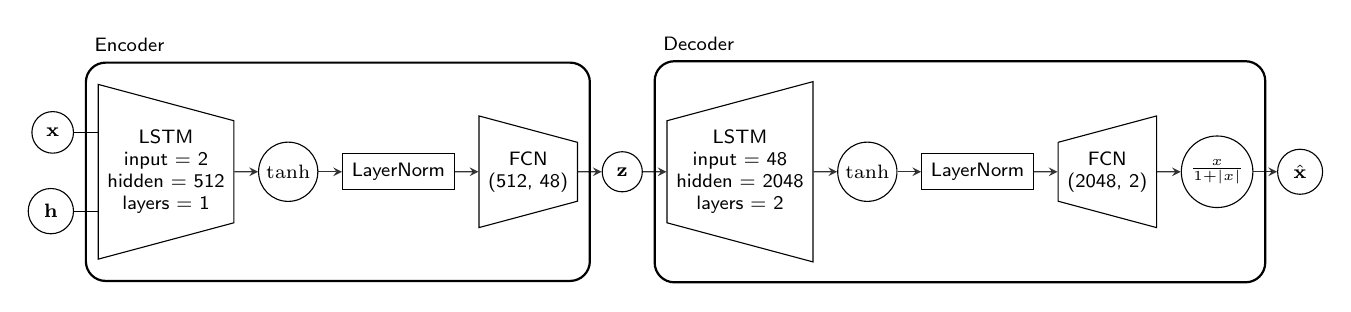
\begin{tikzpicture}[
            input/.style={circle, draw},
            output/.style={circle, draw},
            fcn/.style={rectangle, draw},
            cnn/.style={rectangle, draw},
            rnn/.style={rectangle, draw},
        ]
        {[start chain]
            \node [rnn, ml/encoder, on chain] (lstm_e) {LSTM \\ input = 2 \\ hidden = 512 \\ layers = 1};
            \node [operator, on chain] (tanh_e) {~$\tanh$~};
            \node [fcn, on chain] (layer_norm_e) {LayerNorm};
            \node [fcn, ml/encoder, on chain] (fcn_e) {FCN \\ (512, 48)};
            \node [input, on chain] (z) {$\vec z$};
            \node [input,ml/decoder, on chain] (lstm_d) {LSTM \\ input = 48 \\ hidden = 2048 \\ layers = 2};
            \node [operator, on chain] (tanh_d) {~$\tanh$~};
            \node [fcn, on chain] (layer_norm_d) {LayerNorm};
            \node [fcn, ml/decoder, on chain] (fcn_d) {FCN \\ (2048, 2)};
            \node [operator, on chain] (softsign_d) {~$\frac{x}{1+|x|}$~};
            \node [output, on chain] (x_hat) {$\hat {\vec x}$};
        }
        \coordinate (lstm_e_north_west) at ($(lstm_e.west)+(0,0.5)$);
        \coordinate (lstm_e_south_west) at ($(lstm_e.west)-(0,0.5)$);

        \node [input, left=of lstm_e_north_west] (x) {$\vec x$};
        \draw (x) -- (lstm_e_north_west);
        \node [input, left=of lstm_e_south_west] (hx) {$\vec h$};
        \draw (hx) -- (lstm_e_south_west);

        \node [cell, inner xsep=1.5mm, fit=(lstm_e) (fcn_e)] (encoder_border) {};
        \node[anchor=south west] at (encoder_border.north west) {Encoder};
        \node [cell, inner xsep=1.5mm, fit=(lstm_d) (softsign_d)] (decoder_border) {};
        \node[anchor=south west] at (decoder_border.north west) {Decoder};
    \end{tikzpicture}
    \caption{RAE architecture using LSTMs for encoding and decoding.
        Using an unbalanced architecture, with the decoder being larger than the encoder, enables higher quality reconstruction which results in faster training and better performance.
        Softsign is applied to the decoder output to ensure that values meet the $s_\mathrm{path} \in [-1,1]$ requirement whilst providing close to linear mappings in this range.
    }
    \label{fig:rae:lstm_ae}
\end{figure*}

\section{Model Architecture}
\label{model_architecture}

\begin{figure}[t!]
    \centering
    \begin{subfigure}[b]{0.4\linewidth}
        \centering
        \includegraphics[width=0.7\linewidth]{assets/discrete_mamba.png}
        \caption{
        The Discrete Mamba-2 block \cite{mohawk} modifies the original Mamba-2 architecture by removing both post-convolution activation and pre-output projection normalization. Additionally, the Discrete Mamba-2 sequence mixer eliminates the $\Delta$ discretization parameter and directly projects the $\mathbf{A}$ matrix from the input.
        }
        \label{fig:discrete_mamba}
    \end{subfigure}
    \hspace{0.1\linewidth} % Adjust the spacing
    \begin{subfigure}[b]{0.4\linewidth}
        \centering
        \includegraphics[width=0.62\linewidth]{assets/llamba_architecture.png}
        \caption{Llamba models—Llamba-1B, Llamba-3B, and Llamba-8B—are based on the architecture of their Llama teacher models. Each block comprises two sub-blocks with residual connections:
        (1) RMS Normalization followed by a Discrete Mamba-2 layer.
        (2) RMS Normalization followed by a feed-forward layer.
        }
        \label{fig:llamba_architecture}
    \end{subfigure}
    \caption{Comparison of the Discrete Mamba-2 block and the Llamba architecture.}
    \label{fig:comparison}
\end{figure}

Unlike the Mamba and Mamba-2 architectures, which were designed for training from scratch, \textit{Llamba is directly motivated by architectural distillation}.
In particular, the Mohawk distillation framework involves aligning sub-networks of the model at various levels of granularity (\Cref{sec:distillation}). 
This constraints Llamba to retain the overall architecture of the teacher model, ideally modifying only the attention matrix mixer by replacing it with a subquadratic alternative.

The Llamba models—Llamba-1B, Llamba-3B, and Llamba-8B—comprise 16, 28, and 32 residual Mamba-2 blocks, respectively, followed by feed-forward layers. These models share the tokenizer and vocabulary of Llama-3.1, with hidden dimensions of 2048 for Llamba-1B, 3072 for Llamba-3B, and 4096 for Llamba-8B. 
In addition, Llamba differs from the original Mamba-2 architecture \citep{mamba2} in the following ways (see \Cref{fig:llamba_architecture}):
\begin{itemize}[leftmargin=*]

\item \textbf{Alternating MLP blocks}:
Llamba interleaves Llama’s Gated MLP components between each Mamba-2 mixing layer, unlike Mamba-1 and Mamba-2, which consist solely of SSM blocks.

\item \textbf{Multi-head structure}: Llama-3.x models use grouped-query attention (GQA) \citep{gqa, mqa}, which employs 32 query heads and 8 key-value heads to boost inference speed and reduce the size of the decoding cache. However, Mamba’s recurrent layers don’t rely on a cache, so these optimizations aren’t needed. Instead, \textit{Llamba blocks feature a Multi-Head variant} of Mamba-2 with 32 heads and dimensions of 64, 96, or 128, along with a state size of 64. While this design differs from Mamba-2’s ``multi-value attention'' (MVA) architecture, it still keeps inference costs low.

\item \textbf{Non-linearities}: We remove the normalization before the output projection and the activation after convolution, as these are non-linear operations that do not exist in the attention block and hurts alignment (See \Cref{subsec:mohawk}). 

\item \textbf{Discretization}: Llamba uses \textit{Discrete-Mamba-2}, a variant that projects the matrix $\mathbf{A}$ directly from the input, eliminating the discretization parameters $\Delta$ to better match the inherently discrete attention mechanisms. 
\end{itemize}

Notably, these changes not only facilitate the distillation process but also improve training efficiency. Alternating with MLPs \textbf{reduces the number of temporal mixing layers}, enabling Llamba to achieve faster computation than other models of comparable size (see \Cref{subsec:throughput}). Furthermore, training becomes simpler and more efficient by eliminating normalization-related all-reduce operations.



\section{Practical Implementation Details}
\label{sect:implementation}

\subsection{Cubature}

The integral is calculated using a cubature integration scheme \citep{cools_algorithm_1997} with constrained Delaunay triangulation \citep{chew_constrained_1987} to subdivide $H_t$ into triangles for fast computation. The use of pseudo-continuous over discrete integration has shown to greatly reduce noise in previous work \citep{ewers_enhancing_2024}. Whilst noise can be beneficial to promote exploration, this must be controllable and tunable. Reducing noise in the reward function, where cubature is being used, is critical to maximize learning efficiency else expensive techniques have to be employed \citep{wang_reinforcement_2020}.

\subsubsection{Recurrent Encoder}

\paragraph{Training}

During training the test dataset was unbatched and chunked into $N \sim \mathcal{U}(2, k)$ length sections where $k$ is the length of the longest path in the batch. If $N < k$ then the hidden states would be reused for the next section rather than resetting. This significantly improved the speed of convergence. Automatic mixed precision was used to further increase training times. A no-improvement criterion was used where training would terminate if the amount of epochs since a loss function decrease breaches a patience threshold.

\paragraph{Deployment}

The recurrent encoder, as detailed in Section \ref{sect:rae}, undergoes separate training from the DRL models with its parameters frozen during DRL training. This isolation prevents latent space divergence that could destabilize the learning during online updates. In our implementation, the encoder resides in the observation preprocessing pipeline rather than the policy network itself. This architectural choice minimizes replay buffer memory and compute requirements during training (critical for SAC's experience replay mechanism), though deployment permits alternative configurations.
The two viable deployment strategies are:
\begin{itemize}
    \item Hidden State Propagation: Stores only the encoder's hidden states (including cell state), giving a constant runtime performance per step with fixed memory usage (hidden states).
    \item  Full History Processing: Maintains complete trajectory histories, with the memory requirements and runtime performance growing linearly with the episode length.
\end{itemize}
In this work the former approach - hidden state propagation - is used. The full history processing approach would be required for other techniques such as temporal convolution networks \citep{lea_temporal_2016} or transformers \citep{vaswani_attention_2017}.

\subsection{Further Architecture Details}

The RPPO implementation used in this work is from \citet{raffin_stablebaselines3_2021} which aligns closely with \citet{pleines_generalization_2022}. The 2D convolution kernel inner-model feature extractor for \fsppoconvtwod and \fssacconvtwod is from \citet{mnih_humanlevel_2015}



\begin{table*}[t]
\centering
\fontsize{11pt}{11pt}\selectfont
\begin{tabular}{lllllllllllll}
\toprule
\multicolumn{1}{c}{\textbf{task}} & \multicolumn{2}{c}{\textbf{Mir}} & \multicolumn{2}{c}{\textbf{Lai}} & \multicolumn{2}{c}{\textbf{Ziegen.}} & \multicolumn{2}{c}{\textbf{Cao}} & \multicolumn{2}{c}{\textbf{Alva-Man.}} & \multicolumn{1}{c}{\textbf{avg.}} & \textbf{\begin{tabular}[c]{@{}l@{}}avg.\\ rank\end{tabular}} \\
\multicolumn{1}{c}{\textbf{metrics}} & \multicolumn{1}{c}{\textbf{cor.}} & \multicolumn{1}{c}{\textbf{p-v.}} & \multicolumn{1}{c}{\textbf{cor.}} & \multicolumn{1}{c}{\textbf{p-v.}} & \multicolumn{1}{c}{\textbf{cor.}} & \multicolumn{1}{c}{\textbf{p-v.}} & \multicolumn{1}{c}{\textbf{cor.}} & \multicolumn{1}{c}{\textbf{p-v.}} & \multicolumn{1}{c}{\textbf{cor.}} & \multicolumn{1}{c}{\textbf{p-v.}} &  &  \\ \midrule
\textbf{S-Bleu} & 0.50 & 0.0 & 0.47 & 0.0 & 0.59 & 0.0 & 0.58 & 0.0 & 0.68 & 0.0 & 0.57 & 5.8 \\
\textbf{R-Bleu} & -- & -- & 0.27 & 0.0 & 0.30 & 0.0 & -- & -- & -- & -- & - &  \\
\textbf{S-Meteor} & 0.49 & 0.0 & 0.48 & 0.0 & 0.61 & 0.0 & 0.57 & 0.0 & 0.64 & 0.0 & 0.56 & 6.1 \\
\textbf{R-Meteor} & -- & -- & 0.34 & 0.0 & 0.26 & 0.0 & -- & -- & -- & -- & - &  \\
\textbf{S-Bertscore} & \textbf{0.53} & 0.0 & {\ul 0.80} & 0.0 & \textbf{0.70} & 0.0 & {\ul 0.66} & 0.0 & {\ul0.78} & 0.0 & \textbf{0.69} & \textbf{1.7} \\
\textbf{R-Bertscore} & -- & -- & 0.51 & 0.0 & 0.38 & 0.0 & -- & -- & -- & -- & - &  \\
\textbf{S-Bleurt} & {\ul 0.52} & 0.0 & {\ul 0.80} & 0.0 & 0.60 & 0.0 & \textbf{0.70} & 0.0 & \textbf{0.80} & 0.0 & {\ul 0.68} & {\ul 2.3} \\
\textbf{R-Bleurt} & -- & -- & 0.59 & 0.0 & -0.05 & 0.13 & -- & -- & -- & -- & - &  \\
\textbf{S-Cosine} & 0.51 & 0.0 & 0.69 & 0.0 & {\ul 0.62} & 0.0 & 0.61 & 0.0 & 0.65 & 0.0 & 0.62 & 4.4 \\
\textbf{R-Cosine} & -- & -- & 0.40 & 0.0 & 0.29 & 0.0 & -- & -- & -- & -- & - & \\ \midrule
\textbf{QuestEval} & 0.23 & 0.0 & 0.25 & 0.0 & 0.49 & 0.0 & 0.47 & 0.0 & 0.62 & 0.0 & 0.41 & 9.0 \\
\textbf{LLaMa3} & 0.36 & 0.0 & \textbf{0.84} & 0.0 & {\ul{0.62}} & 0.0 & 0.61 & 0.0 &  0.76 & 0.0 & 0.64 & 3.6 \\
\textbf{our (3b)} & 0.49 & 0.0 & 0.73 & 0.0 & 0.54 & 0.0 & 0.53 & 0.0 & 0.7 & 0.0 & 0.60 & 5.8 \\
\textbf{our (8b)} & 0.48 & 0.0 & 0.73 & 0.0 & 0.52 & 0.0 & 0.53 & 0.0 & 0.7 & 0.0 & 0.59 & 6.3 \\  \bottomrule
\end{tabular}
\caption{Pearson correlation on human evaluation on system output. `R-': reference-based. `S-': source-based.}
\label{tab:sys}
\end{table*}



\begin{table}%[]
\centering
\fontsize{11pt}{11pt}\selectfont
\begin{tabular}{llllll}
\toprule
\multicolumn{1}{c}{\textbf{task}} & \multicolumn{1}{c}{\textbf{Lai}} & \multicolumn{1}{c}{\textbf{Zei.}} & \multicolumn{1}{c}{\textbf{Scia.}} & \textbf{} & \textbf{} \\ 
\multicolumn{1}{c}{\textbf{metrics}} & \multicolumn{1}{c}{\textbf{cor.}} & \multicolumn{1}{c}{\textbf{cor.}} & \multicolumn{1}{c}{\textbf{cor.}} & \textbf{avg.} & \textbf{\begin{tabular}[c]{@{}l@{}}avg.\\ rank\end{tabular}} \\ \midrule
\textbf{S-Bleu} & 0.40 & 0.40 & 0.19* & 0.33 & 7.67 \\
\textbf{S-Meteor} & 0.41 & 0.42 & 0.16* & 0.33 & 7.33 \\
\textbf{S-BertS.} & {\ul0.58} & 0.47 & 0.31 & 0.45 & 3.67 \\
\textbf{S-Bleurt} & 0.45 & {\ul 0.54} & {\ul 0.37} & 0.45 & {\ul 3.33} \\
\textbf{S-Cosine} & 0.56 & 0.52 & 0.3 & {\ul 0.46} & {\ul 3.33} \\ \midrule
\textbf{QuestE.} & 0.27 & 0.35 & 0.06* & 0.23 & 9.00 \\
\textbf{LlaMA3} & \textbf{0.6} & \textbf{0.67} & \textbf{0.51} & \textbf{0.59} & \textbf{1.0} \\
\textbf{Our (3b)} & 0.51 & 0.49 & 0.23* & 0.39 & 4.83 \\
\textbf{Our (8b)} & 0.52 & 0.49 & 0.22* & 0.43 & 4.83 \\ \bottomrule
\end{tabular}
\caption{Pearson correlation on human ratings on reference output. *not significant; we cannot reject the null hypothesis of zero correlation}
\label{tab:ref}
\end{table}


\begin{table*}%[]
\centering
\fontsize{11pt}{11pt}\selectfont
\begin{tabular}{lllllllll}
\toprule
\textbf{task} & \multicolumn{1}{c}{\textbf{ALL}} & \multicolumn{1}{c}{\textbf{sentiment}} & \multicolumn{1}{c}{\textbf{detoxify}} & \multicolumn{1}{c}{\textbf{catchy}} & \multicolumn{1}{c}{\textbf{polite}} & \multicolumn{1}{c}{\textbf{persuasive}} & \multicolumn{1}{c}{\textbf{formal}} & \textbf{\begin{tabular}[c]{@{}l@{}}avg. \\ rank\end{tabular}} \\
\textbf{metrics} & \multicolumn{1}{c}{\textbf{cor.}} & \multicolumn{1}{c}{\textbf{cor.}} & \multicolumn{1}{c}{\textbf{cor.}} & \multicolumn{1}{c}{\textbf{cor.}} & \multicolumn{1}{c}{\textbf{cor.}} & \multicolumn{1}{c}{\textbf{cor.}} & \multicolumn{1}{c}{\textbf{cor.}} &  \\ \midrule
\textbf{S-Bleu} & -0.17 & -0.82 & -0.45 & -0.12* & -0.1* & -0.05 & -0.21 & 8.42 \\
\textbf{R-Bleu} & - & -0.5 & -0.45 &  &  &  &  &  \\
\textbf{S-Meteor} & -0.07* & -0.55 & -0.4 & -0.01* & 0.1* & -0.16 & -0.04* & 7.67 \\
\textbf{R-Meteor} & - & -0.17* & -0.39 & - & - & - & - & - \\
\textbf{S-BertScore} & 0.11 & -0.38 & -0.07* & -0.17* & 0.28 & 0.12 & 0.25 & 6.0 \\
\textbf{R-BertScore} & - & -0.02* & -0.21* & - & - & - & - & - \\
\textbf{S-Bleurt} & 0.29 & 0.05* & 0.45 & 0.06* & 0.29 & 0.23 & 0.46 & 4.2 \\
\textbf{R-Bleurt} & - &  0.21 & 0.38 & - & - & - & - & - \\
\textbf{S-Cosine} & 0.01* & -0.5 & -0.13* & -0.19* & 0.05* & -0.05* & 0.15* & 7.42 \\
\textbf{R-Cosine} & - & -0.11* & -0.16* & - & - & - & - & - \\ \midrule
\textbf{QuestEval} & 0.21 & {\ul{0.29}} & 0.23 & 0.37 & 0.19* & 0.35 & 0.14* & 4.67 \\
\textbf{LlaMA3} & \textbf{0.82} & \textbf{0.80} & \textbf{0.72} & \textbf{0.84} & \textbf{0.84} & \textbf{0.90} & \textbf{0.88} & \textbf{1.00} \\
\textbf{Our (3b)} & 0.47 & -0.11* & 0.37 & 0.61 & 0.53 & 0.54 & 0.66 & 3.5 \\
\textbf{Our (8b)} & {\ul{0.57}} & 0.09* & {\ul 0.49} & {\ul 0.72} & {\ul 0.64} & {\ul 0.62} & {\ul 0.67} & {\ul 2.17} \\ \bottomrule
\end{tabular}
\caption{Pearson correlation on human ratings on our constructed test set. 'R-': reference-based. 'S-': source-based. *not significant; we cannot reject the null hypothesis of zero correlation}
\label{tab:con}
\end{table*}

\section{Results}
We benchmark the different metrics on the different datasets using correlation to human judgement. For content preservation, we show results split on data with system output, reference output and our constructed test set: we show that the data source for evaluation leads to different conclusions on the metrics. In addition, we examine whether the metrics can rank style transfer systems similar to humans. On style strength, we likewise show correlations between human judgment and zero-shot evaluation approaches. When applicable, we summarize results by reporting the average correlation. And the average ranking of the metric per dataset (by ranking which metric obtains the highest correlation to human judgement per dataset). 

\subsection{Content preservation}
\paragraph{How do data sources affect the conclusion on best metric?}
The conclusions about the metrics' performance change radically depending on whether we use system output data, reference output, or our constructed test set. Ideally, a good metric correlates highly with humans on any data source. Ideally, for meta-evaluation, a metric should correlate consistently across all data sources, but the following shows that the correlations indicate different things, and the conclusion on the best metric should be drawn carefully.

Looking at the metrics correlations with humans on the data source with system output (Table~\ref{tab:sys}), we see a relatively high correlation for many of the metrics on many tasks. The overall best metrics are S-BertScore and S-BLEURT (avg+avg rank). We see no notable difference in our method of using the 3B or 8B model as the backbone.

Examining the average correlations based on data with reference output (Table~\ref{tab:ref}), now the zero-shoot prompting with LlaMA3 70B is the best-performing approach ($0.59$ avg). Tied for second place are source-based cosine embedding ($0.46$ avg), BLEURT ($0.45$ avg) and BertScore ($0.45$ avg). Our method follows on a 5. place: here, the 8b version (($0.43$ avg)) shows a bit stronger results than 3b ($0.39$ avg). The fact that the conclusions change, whether looking at reference or system output, confirms the observations made by \citet{scialom-etal-2021-questeval} on simplicity transfer.   

Now consider the results on our test set (Table~\ref{tab:con}): Several metrics show low or no correlation; we even see a significantly negative correlation for some metrics on ALL (BLEU) and for specific subparts of our test set for BLEU, Meteor, BertScore, Cosine. On the other end, LlaMA3 70B is again performing best, showing strong results ($0.82$ in ALL). The runner-up is now our 8B method, with a gap to the 3B version ($0.57$ vs $0.47$ in ALL). Note our method still shows zero correlation for the sentiment task. After, ranks BLEURT ($0.29$), QuestEval ($0.21$), BertScore ($0.11$), Cosine ($0.01$).  

On our test set, we find that some metrics that correlate relatively well on the other datasets, now exhibit low correlation. Hence, with our test set, we can now support the logical reasoning with data evidence: Evaluation of content preservation for style transfer needs to take the style shift into account. This conclusion could not be drawn using the existing data sources: We hypothesise that for the data with system-based output, successful output happens to be very similar to the source sentence and vice versa, and reference-based output might not contain server mistakes as they are gold references. Thus, none of the existing data sources tests the limits of the metrics.  


\paragraph{How do reference-based metrics compare to source-based ones?} Reference-based metrics show a lower correlation than the source-based counterpart for all metrics on both datasets with ratings on references (Table~\ref{tab:sys}). As discussed previously, reference-based metrics for style transfer have the drawback that many different good solutions on a rewrite might exist and not only one similar to a reference.


\paragraph{How well can the metrics rank the performance of style transfer methods?}
We compare the metrics' ability to judge the best style transfer methods w.r.t. the human annotations: Several of the data sources contain samples from different style transfer systems. In order to use metrics to assess the quality of the style transfer system, metrics should correctly find the best-performing system. Hence, we evaluate whether the metrics for content preservation provide the same system ranking as human evaluators. We take the mean of the score for every output on each system and the mean of the human annotations; we compare the systems using the Kendall's Tau correlation. 

We find only the evaluation using the dataset Mir, Lai, and Ziegen to result in significant correlations, probably because of sparsity in a number of system tests (App.~\ref{app:dataset}). Our method (8b) is the only metric providing a perfect ranking of the style transfer system on the Lai data, and Llama3 70B the only one on the Ziegen data. Results in App.~\ref{app:results}. 


\subsection{Style strength results}
%Evaluating style strengths is a challenging task. 
Llama3 70B shows better overall results than our method. However, our method scores higher than Llama3 70B on 2 out of 6 datasets, but it also exhibits zero correlation on one task (Table~\ref{tab:styleresults}).%More work i s needed on evaluating style strengths. 
 
\begin{table}%[]
\fontsize{11pt}{11pt}\selectfont
\begin{tabular}{lccc}
\toprule
\multicolumn{1}{c}{\textbf{}} & \textbf{LlaMA3} & \textbf{Our (3b)} & \textbf{Our (8b)} \\ \midrule
\textbf{Mir} & 0.46 & 0.54 & \textbf{0.57} \\
\textbf{Lai} & \textbf{0.57} & 0.18 & 0.19 \\
\textbf{Ziegen.} & 0.25 & 0.27 & \textbf{0.32} \\
\textbf{Alva-M.} & \textbf{0.59} & 0.03* & 0.02* \\
\textbf{Scialom} & \textbf{0.62} & 0.45 & 0.44 \\
\textbf{\begin{tabular}[c]{@{}l@{}}Our Test\end{tabular}} & \textbf{0.63} & 0.46 & 0.48 \\ \bottomrule
\end{tabular}
\caption{Style strength: Pearson correlation to human ratings. *not significant; we cannot reject the null hypothesis of zero corelation}
\label{tab:styleresults}
\end{table}

\subsection{Ablation}
We conduct several runs of the methods using LLMs with variations in instructions/prompts (App.~\ref{app:method}). We observe that the lower the correlation on a task, the higher the variation between the different runs. For our method, we only observe low variance between the runs.
None of the variations leads to different conclusions of the meta-evaluation. Results in App.~\ref{app:results}.

\section{Discussion of Assumptions}\label{sec:discussion}
In this paper, we have made several assumptions for the sake of clarity and simplicity. In this section, we discuss the rationale behind these assumptions, the extent to which these assumptions hold in practice, and the consequences for our protocol when these assumptions hold.

\subsection{Assumptions on the Demand}

There are two simplifying assumptions we make about the demand. First, we assume the demand at any time is relatively small compared to the channel capacities. Second, we take the demand to be constant over time. We elaborate upon both these points below.

\paragraph{Small demands} The assumption that demands are small relative to channel capacities is made precise in \eqref{eq:large_capacity_assumption}. This assumption simplifies two major aspects of our protocol. First, it largely removes congestion from consideration. In \eqref{eq:primal_problem}, there is no constraint ensuring that total flow in both directions stays below capacity--this is always met. Consequently, there is no Lagrange multiplier for congestion and no congestion pricing; only imbalance penalties apply. In contrast, protocols in \cite{sivaraman2020high, varma2021throughput, wang2024fence} include congestion fees due to explicit congestion constraints. Second, the bound \eqref{eq:large_capacity_assumption} ensures that as long as channels remain balanced, the network can always meet demand, no matter how the demand is routed. Since channels can rebalance when necessary, they never drop transactions. This allows prices and flows to adjust as per the equations in \eqref{eq:algorithm}, which makes it easier to prove the protocol's convergence guarantees. This also preserves the key property that a channel's price remains proportional to net money flow through it.

In practice, payment channel networks are used most often for micro-payments, for which on-chain transactions are prohibitively expensive; large transactions typically take place directly on the blockchain. For example, according to \cite{river2023lightning}, the average channel capacity is roughly $0.1$ BTC ($5,000$ BTC distributed over $50,000$ channels), while the average transaction amount is less than $0.0004$ BTC ($44.7k$ satoshis). Thus, the small demand assumption is not too unrealistic. Additionally, the occasional large transaction can be treated as a sequence of smaller transactions by breaking it into packets and executing each packet serially (as done by \cite{sivaraman2020high}).
Lastly, a good path discovery process that favors large capacity channels over small capacity ones can help ensure that the bound in \eqref{eq:large_capacity_assumption} holds.

\paragraph{Constant demands} 
In this work, we assume that any transacting pair of nodes have a steady transaction demand between them (see Section \ref{sec:transaction_requests}). Making this assumption is necessary to obtain the kind of guarantees that we have presented in this paper. Unless the demand is steady, it is unreasonable to expect that the flows converge to a steady value. Weaker assumptions on the demand lead to weaker guarantees. For example, with the more general setting of stochastic, but i.i.d. demand between any two nodes, \cite{varma2021throughput} shows that the channel queue lengths are bounded in expectation. If the demand can be arbitrary, then it is very hard to get any meaningful performance guarantees; \cite{wang2024fence} shows that even for a single bidirectional channel, the competitive ratio is infinite. Indeed, because a PCN is a decentralized system and decisions must be made based on local information alone, it is difficult for the network to find the optimal detailed balance flow at every time step with a time-varying demand.  With a steady demand, the network can discover the optimal flows in a reasonably short time, as our work shows.

We view the constant demand assumption as an approximation for a more general demand process that could be piece-wise constant, stochastic, or both (see simulations in Figure \ref{fig:five_nodes_variable_demand}).
We believe it should be possible to merge ideas from our work and \cite{varma2021throughput} to provide guarantees in a setting with random demands with arbitrary means. We leave this for future work. In addition, our work suggests that a reasonable method of handling stochastic demands is to queue the transaction requests \textit{at the source node} itself. This queuing action should be viewed in conjunction with flow-control. Indeed, a temporarily high unidirectional demand would raise prices for the sender, incentivizing the sender to stop sending the transactions. If the sender queues the transactions, they can send them later when prices drop. This form of queuing does not require any overhaul of the basic PCN infrastructure and is therefore simpler to implement than per-channel queues as suggested by \cite{sivaraman2020high} and \cite{varma2021throughput}.

\subsection{The Incentive of Channels}
The actions of the channels as prescribed by the DEBT control protocol can be summarized as follows. Channels adjust their prices in proportion to the net flow through them. They rebalance themselves whenever necessary and execute any transaction request that has been made of them. We discuss both these aspects below.

\paragraph{On Prices}
In this work, the exclusive role of channel prices is to ensure that the flows through each channel remains balanced. In practice, it would be important to include other components in a channel's price/fee as well: a congestion price  and an incentive price. The congestion price, as suggested by \cite{varma2021throughput}, would depend on the total flow of transactions through the channel, and would incentivize nodes to balance the load over different paths. The incentive price, which is commonly used in practice \cite{river2023lightning}, is necessary to provide channels with an incentive to serve as an intermediary for different channels. In practice, we expect both these components to be smaller than the imbalance price. Consequently, we expect the behavior of our protocol to be similar to our theoretical results even with these additional prices.

A key aspect of our protocol is that channel fees are allowed to be negative. Although the original Lightning network whitepaper \cite{poon2016bitcoin} suggests that negative channel prices may be a good solution to promote rebalancing, the idea of negative prices in not very popular in the literature. To our knowledge, the only prior work with this feature is \cite{varma2021throughput}. Indeed, in papers such as \cite{van2021merchant} and \cite{wang2024fence}, the price function is explicitly modified such that the channel price is never negative. The results of our paper show the benefits of negative prices. For one, in steady state, equal flows in both directions ensure that a channel doesn't loose any money (the other price components mentioned above ensure that the channel will only gain money). More importantly, negative prices are important to ensure that the protocol selectively stifles acyclic flows while allowing circulations to flow. Indeed, in the example of Section \ref{sec:flow_control_example}, the flows between nodes $A$ and $C$ are left on only because the large positive price over one channel is canceled by the corresponding negative price over the other channel, leading to a net zero price.

Lastly, observe that in the DEBT control protocol, the price charged by a channel does not depend on its capacity. This is a natural consequence of the price being the Lagrange multiplier for the net-zero flow constraint, which also does not depend on the channel capacity. In contrast, in many other works, the imbalance price is normalized by the channel capacity \cite{ren2018optimal, lin2020funds, wang2024fence}; this is shown to work well in practice. The rationale for such a price structure is explained well in \cite{wang2024fence}, where this fee is derived with the aim of always maintaining some balance (liquidity) at each end of every channel. This is a reasonable aim if a channel is to never rebalance itself; the experiments of the aforementioned papers are conducted in such a regime. In this work, however, we allow the channels to rebalance themselves a few times in order to settle on a detailed balance flow. This is because our focus is on the long-term steady state performance of the protocol. This difference in perspective also shows up in how the price depends on the channel imbalance. \cite{lin2020funds} and \cite{wang2024fence} advocate for strictly convex prices whereas this work and \cite{varma2021throughput} propose linear prices.

\paragraph{On Rebalancing} 
Recall that the DEBT control protocol ensures that the flows in the network converge to a detailed balance flow, which can be sustained perpetually without any rebalancing. However, during the transient phase (before convergence), channels may have to perform on-chain rebalancing a few times. Since rebalancing is an expensive operation, it is worthwhile discussing methods by which channels can reduce the extent of rebalancing. One option for the channels to reduce the extent of rebalancing is to increase their capacity; however, this comes at the cost of locking in more capital. Each channel can decide for itself the optimum amount of capital to lock in. Another option, which we discuss in Section \ref{sec:five_node}, is for channels to increase the rate $\gamma$ at which they adjust prices. 

Ultimately, whether or not it is beneficial for a channel to rebalance depends on the time-horizon under consideration. Our protocol is based on the assumption that the demand remains steady for a long period of time. If this is indeed the case, it would be worthwhile for a channel to rebalance itself as it can make up this cost through the incentive fees gained from the flow of transactions through it in steady state. If a channel chooses not to rebalance itself, however, there is a risk of being trapped in a deadlock, which is suboptimal for not only the nodes but also the channel.

\section{Conclusion}
This work presents DEBT control: a protocol for payment channel networks that uses source routing and flow control based on channel prices. The protocol is derived by posing a network utility maximization problem and analyzing its dual minimization. It is shown that under steady demands, the protocol guides the network to an optimal, sustainable point. Simulations show its robustness to demand variations. The work demonstrates that simple protocols with strong theoretical guarantees are possible for PCNs and we hope it inspires further theoretical research in this direction.

\section{Conclusion}
In this work, we propose a simple yet effective approach, called SMILE, for graph few-shot learning with fewer tasks. Specifically, we introduce a novel dual-level mixup strategy, including within-task and across-task mixup, for enriching the diversity of nodes within each task and the diversity of tasks. Also, we incorporate the degree-based prior information to learn expressive node embeddings. Theoretically, we prove that SMILE effectively enhances the model's generalization performance. Empirically, we conduct extensive experiments on multiple benchmarks and the results suggest that SMILE significantly outperforms other baselines, including both in-domain and cross-domain few-shot settings.

\bibliography{references}

\subsection{Lloyd-Max Algorithm}
\label{subsec:Lloyd-Max}
For a given quantization bitwidth $B$ and an operand $\bm{X}$, the Lloyd-Max algorithm finds $2^B$ quantization levels $\{\hat{x}_i\}_{i=1}^{2^B}$ such that quantizing $\bm{X}$ by rounding each scalar in $\bm{X}$ to the nearest quantization level minimizes the quantization MSE. 

The algorithm starts with an initial guess of quantization levels and then iteratively computes quantization thresholds $\{\tau_i\}_{i=1}^{2^B-1}$ and updates quantization levels $\{\hat{x}_i\}_{i=1}^{2^B}$. Specifically, at iteration $n$, thresholds are set to the midpoints of the previous iteration's levels:
\begin{align*}
    \tau_i^{(n)}=\frac{\hat{x}_i^{(n-1)}+\hat{x}_{i+1}^{(n-1)}}2 \text{ for } i=1\ldots 2^B-1
\end{align*}
Subsequently, the quantization levels are re-computed as conditional means of the data regions defined by the new thresholds:
\begin{align*}
    \hat{x}_i^{(n)}=\mathbb{E}\left[ \bm{X} \big| \bm{X}\in [\tau_{i-1}^{(n)},\tau_i^{(n)}] \right] \text{ for } i=1\ldots 2^B
\end{align*}
where to satisfy boundary conditions we have $\tau_0=-\infty$ and $\tau_{2^B}=\infty$. The algorithm iterates the above steps until convergence.

Figure \ref{fig:lm_quant} compares the quantization levels of a $7$-bit floating point (E3M3) quantizer (left) to a $7$-bit Lloyd-Max quantizer (right) when quantizing a layer of weights from the GPT3-126M model at a per-tensor granularity. As shown, the Lloyd-Max quantizer achieves substantially lower quantization MSE. Further, Table \ref{tab:FP7_vs_LM7} shows the superior perplexity achieved by Lloyd-Max quantizers for bitwidths of $7$, $6$ and $5$. The difference between the quantizers is clear at 5 bits, where per-tensor FP quantization incurs a drastic and unacceptable increase in perplexity, while Lloyd-Max quantization incurs a much smaller increase. Nevertheless, we note that even the optimal Lloyd-Max quantizer incurs a notable ($\sim 1.5$) increase in perplexity due to the coarse granularity of quantization. 

\begin{figure}[h]
  \centering
  \includegraphics[width=0.7\linewidth]{sections/figures/LM7_FP7.pdf}
  \caption{\small Quantization levels and the corresponding quantization MSE of Floating Point (left) vs Lloyd-Max (right) Quantizers for a layer of weights in the GPT3-126M model.}
  \label{fig:lm_quant}
\end{figure}

\begin{table}[h]\scriptsize
\begin{center}
\caption{\label{tab:FP7_vs_LM7} \small Comparing perplexity (lower is better) achieved by floating point quantizers and Lloyd-Max quantizers on a GPT3-126M model for the Wikitext-103 dataset.}
\begin{tabular}{c|cc|c}
\hline
 \multirow{2}{*}{\textbf{Bitwidth}} & \multicolumn{2}{|c|}{\textbf{Floating-Point Quantizer}} & \textbf{Lloyd-Max Quantizer} \\
 & Best Format & Wikitext-103 Perplexity & Wikitext-103 Perplexity \\
\hline
7 & E3M3 & 18.32 & 18.27 \\
6 & E3M2 & 19.07 & 18.51 \\
5 & E4M0 & 43.89 & 19.71 \\
\hline
\end{tabular}
\end{center}
\end{table}

\subsection{Proof of Local Optimality of LO-BCQ}
\label{subsec:lobcq_opt_proof}
For a given block $\bm{b}_j$, the quantization MSE during LO-BCQ can be empirically evaluated as $\frac{1}{L_b}\lVert \bm{b}_j- \bm{\hat{b}}_j\rVert^2_2$ where $\bm{\hat{b}}_j$ is computed from equation (\ref{eq:clustered_quantization_definition}) as $C_{f(\bm{b}_j)}(\bm{b}_j)$. Further, for a given block cluster $\mathcal{B}_i$, we compute the quantization MSE as $\frac{1}{|\mathcal{B}_{i}|}\sum_{\bm{b} \in \mathcal{B}_{i}} \frac{1}{L_b}\lVert \bm{b}- C_i^{(n)}(\bm{b})\rVert^2_2$. Therefore, at the end of iteration $n$, we evaluate the overall quantization MSE $J^{(n)}$ for a given operand $\bm{X}$ composed of $N_c$ block clusters as:
\begin{align*}
    \label{eq:mse_iter_n}
    J^{(n)} = \frac{1}{N_c} \sum_{i=1}^{N_c} \frac{1}{|\mathcal{B}_{i}^{(n)}|}\sum_{\bm{v} \in \mathcal{B}_{i}^{(n)}} \frac{1}{L_b}\lVert \bm{b}- B_i^{(n)}(\bm{b})\rVert^2_2
\end{align*}

At the end of iteration $n$, the codebooks are updated from $\mathcal{C}^{(n-1)}$ to $\mathcal{C}^{(n)}$. However, the mapping of a given vector $\bm{b}_j$ to quantizers $\mathcal{C}^{(n)}$ remains as  $f^{(n)}(\bm{b}_j)$. At the next iteration, during the vector clustering step, $f^{(n+1)}(\bm{b}_j)$ finds new mapping of $\bm{b}_j$ to updated codebooks $\mathcal{C}^{(n)}$ such that the quantization MSE over the candidate codebooks is minimized. Therefore, we obtain the following result for $\bm{b}_j$:
\begin{align*}
\frac{1}{L_b}\lVert \bm{b}_j - C_{f^{(n+1)}(\bm{b}_j)}^{(n)}(\bm{b}_j)\rVert^2_2 \le \frac{1}{L_b}\lVert \bm{b}_j - C_{f^{(n)}(\bm{b}_j)}^{(n)}(\bm{b}_j)\rVert^2_2
\end{align*}

That is, quantizing $\bm{b}_j$ at the end of the block clustering step of iteration $n+1$ results in lower quantization MSE compared to quantizing at the end of iteration $n$. Since this is true for all $\bm{b} \in \bm{X}$, we assert the following:
\begin{equation}
\begin{split}
\label{eq:mse_ineq_1}
    \tilde{J}^{(n+1)} &= \frac{1}{N_c} \sum_{i=1}^{N_c} \frac{1}{|\mathcal{B}_{i}^{(n+1)}|}\sum_{\bm{b} \in \mathcal{B}_{i}^{(n+1)}} \frac{1}{L_b}\lVert \bm{b} - C_i^{(n)}(b)\rVert^2_2 \le J^{(n)}
\end{split}
\end{equation}
where $\tilde{J}^{(n+1)}$ is the the quantization MSE after the vector clustering step at iteration $n+1$.

Next, during the codebook update step (\ref{eq:quantizers_update}) at iteration $n+1$, the per-cluster codebooks $\mathcal{C}^{(n)}$ are updated to $\mathcal{C}^{(n+1)}$ by invoking the Lloyd-Max algorithm \citep{Lloyd}. We know that for any given value distribution, the Lloyd-Max algorithm minimizes the quantization MSE. Therefore, for a given vector cluster $\mathcal{B}_i$ we obtain the following result:

\begin{equation}
    \frac{1}{|\mathcal{B}_{i}^{(n+1)}|}\sum_{\bm{b} \in \mathcal{B}_{i}^{(n+1)}} \frac{1}{L_b}\lVert \bm{b}- C_i^{(n+1)}(\bm{b})\rVert^2_2 \le \frac{1}{|\mathcal{B}_{i}^{(n+1)}|}\sum_{\bm{b} \in \mathcal{B}_{i}^{(n+1)}} \frac{1}{L_b}\lVert \bm{b}- C_i^{(n)}(\bm{b})\rVert^2_2
\end{equation}

The above equation states that quantizing the given block cluster $\mathcal{B}_i$ after updating the associated codebook from $C_i^{(n)}$ to $C_i^{(n+1)}$ results in lower quantization MSE. Since this is true for all the block clusters, we derive the following result: 
\begin{equation}
\begin{split}
\label{eq:mse_ineq_2}
     J^{(n+1)} &= \frac{1}{N_c} \sum_{i=1}^{N_c} \frac{1}{|\mathcal{B}_{i}^{(n+1)}|}\sum_{\bm{b} \in \mathcal{B}_{i}^{(n+1)}} \frac{1}{L_b}\lVert \bm{b}- C_i^{(n+1)}(\bm{b})\rVert^2_2  \le \tilde{J}^{(n+1)}   
\end{split}
\end{equation}

Following (\ref{eq:mse_ineq_1}) and (\ref{eq:mse_ineq_2}), we find that the quantization MSE is non-increasing for each iteration, that is, $J^{(1)} \ge J^{(2)} \ge J^{(3)} \ge \ldots \ge J^{(M)}$ where $M$ is the maximum number of iterations. 
%Therefore, we can say that if the algorithm converges, then it must be that it has converged to a local minimum. 
\hfill $\blacksquare$


\begin{figure}
    \begin{center}
    \includegraphics[width=0.5\textwidth]{sections//figures/mse_vs_iter.pdf}
    \end{center}
    \caption{\small NMSE vs iterations during LO-BCQ compared to other block quantization proposals}
    \label{fig:nmse_vs_iter}
\end{figure}

Figure \ref{fig:nmse_vs_iter} shows the empirical convergence of LO-BCQ across several block lengths and number of codebooks. Also, the MSE achieved by LO-BCQ is compared to baselines such as MXFP and VSQ. As shown, LO-BCQ converges to a lower MSE than the baselines. Further, we achieve better convergence for larger number of codebooks ($N_c$) and for a smaller block length ($L_b$), both of which increase the bitwidth of BCQ (see Eq \ref{eq:bitwidth_bcq}).


\subsection{Additional Accuracy Results}
%Table \ref{tab:lobcq_config} lists the various LOBCQ configurations and their corresponding bitwidths.
\begin{table}
\setlength{\tabcolsep}{4.75pt}
\begin{center}
\caption{\label{tab:lobcq_config} Various LO-BCQ configurations and their bitwidths.}
\begin{tabular}{|c||c|c|c|c||c|c||c|} 
\hline
 & \multicolumn{4}{|c||}{$L_b=8$} & \multicolumn{2}{|c||}{$L_b=4$} & $L_b=2$ \\
 \hline
 \backslashbox{$L_A$\kern-1em}{\kern-1em$N_c$} & 2 & 4 & 8 & 16 & 2 & 4 & 2 \\
 \hline
 64 & 4.25 & 4.375 & 4.5 & 4.625 & 4.375 & 4.625 & 4.625\\
 \hline
 32 & 4.375 & 4.5 & 4.625& 4.75 & 4.5 & 4.75 & 4.75 \\
 \hline
 16 & 4.625 & 4.75& 4.875 & 5 & 4.75 & 5 & 5 \\
 \hline
\end{tabular}
\end{center}
\end{table}

%\subsection{Perplexity achieved by various LO-BCQ configurations on Wikitext-103 dataset}

\begin{table} \centering
\begin{tabular}{|c||c|c|c|c||c|c||c|} 
\hline
 $L_b \rightarrow$& \multicolumn{4}{c||}{8} & \multicolumn{2}{c||}{4} & 2\\
 \hline
 \backslashbox{$L_A$\kern-1em}{\kern-1em$N_c$} & 2 & 4 & 8 & 16 & 2 & 4 & 2  \\
 %$N_c \rightarrow$ & 2 & 4 & 8 & 16 & 2 & 4 & 2 \\
 \hline
 \hline
 \multicolumn{8}{c}{GPT3-1.3B (FP32 PPL = 9.98)} \\ 
 \hline
 \hline
 64 & 10.40 & 10.23 & 10.17 & 10.15 &  10.28 & 10.18 & 10.19 \\
 \hline
 32 & 10.25 & 10.20 & 10.15 & 10.12 &  10.23 & 10.17 & 10.17 \\
 \hline
 16 & 10.22 & 10.16 & 10.10 & 10.09 &  10.21 & 10.14 & 10.16 \\
 \hline
  \hline
 \multicolumn{8}{c}{GPT3-8B (FP32 PPL = 7.38)} \\ 
 \hline
 \hline
 64 & 7.61 & 7.52 & 7.48 &  7.47 &  7.55 &  7.49 & 7.50 \\
 \hline
 32 & 7.52 & 7.50 & 7.46 &  7.45 &  7.52 &  7.48 & 7.48  \\
 \hline
 16 & 7.51 & 7.48 & 7.44 &  7.44 &  7.51 &  7.49 & 7.47  \\
 \hline
\end{tabular}
\caption{\label{tab:ppl_gpt3_abalation} Wikitext-103 perplexity across GPT3-1.3B and 8B models.}
\end{table}

\begin{table} \centering
\begin{tabular}{|c||c|c|c|c||} 
\hline
 $L_b \rightarrow$& \multicolumn{4}{c||}{8}\\
 \hline
 \backslashbox{$L_A$\kern-1em}{\kern-1em$N_c$} & 2 & 4 & 8 & 16 \\
 %$N_c \rightarrow$ & 2 & 4 & 8 & 16 & 2 & 4 & 2 \\
 \hline
 \hline
 \multicolumn{5}{|c|}{Llama2-7B (FP32 PPL = 5.06)} \\ 
 \hline
 \hline
 64 & 5.31 & 5.26 & 5.19 & 5.18  \\
 \hline
 32 & 5.23 & 5.25 & 5.18 & 5.15  \\
 \hline
 16 & 5.23 & 5.19 & 5.16 & 5.14  \\
 \hline
 \multicolumn{5}{|c|}{Nemotron4-15B (FP32 PPL = 5.87)} \\ 
 \hline
 \hline
 64  & 6.3 & 6.20 & 6.13 & 6.08  \\
 \hline
 32  & 6.24 & 6.12 & 6.07 & 6.03  \\
 \hline
 16  & 6.12 & 6.14 & 6.04 & 6.02  \\
 \hline
 \multicolumn{5}{|c|}{Nemotron4-340B (FP32 PPL = 3.48)} \\ 
 \hline
 \hline
 64 & 3.67 & 3.62 & 3.60 & 3.59 \\
 \hline
 32 & 3.63 & 3.61 & 3.59 & 3.56 \\
 \hline
 16 & 3.61 & 3.58 & 3.57 & 3.55 \\
 \hline
\end{tabular}
\caption{\label{tab:ppl_llama7B_nemo15B} Wikitext-103 perplexity compared to FP32 baseline in Llama2-7B and Nemotron4-15B, 340B models}
\end{table}

%\subsection{Perplexity achieved by various LO-BCQ configurations on MMLU dataset}


\begin{table} \centering
\begin{tabular}{|c||c|c|c|c||c|c|c|c|} 
\hline
 $L_b \rightarrow$& \multicolumn{4}{c||}{8} & \multicolumn{4}{c||}{8}\\
 \hline
 \backslashbox{$L_A$\kern-1em}{\kern-1em$N_c$} & 2 & 4 & 8 & 16 & 2 & 4 & 8 & 16  \\
 %$N_c \rightarrow$ & 2 & 4 & 8 & 16 & 2 & 4 & 2 \\
 \hline
 \hline
 \multicolumn{5}{|c|}{Llama2-7B (FP32 Accuracy = 45.8\%)} & \multicolumn{4}{|c|}{Llama2-70B (FP32 Accuracy = 69.12\%)} \\ 
 \hline
 \hline
 64 & 43.9 & 43.4 & 43.9 & 44.9 & 68.07 & 68.27 & 68.17 & 68.75 \\
 \hline
 32 & 44.5 & 43.8 & 44.9 & 44.5 & 68.37 & 68.51 & 68.35 & 68.27  \\
 \hline
 16 & 43.9 & 42.7 & 44.9 & 45 & 68.12 & 68.77 & 68.31 & 68.59  \\
 \hline
 \hline
 \multicolumn{5}{|c|}{GPT3-22B (FP32 Accuracy = 38.75\%)} & \multicolumn{4}{|c|}{Nemotron4-15B (FP32 Accuracy = 64.3\%)} \\ 
 \hline
 \hline
 64 & 36.71 & 38.85 & 38.13 & 38.92 & 63.17 & 62.36 & 63.72 & 64.09 \\
 \hline
 32 & 37.95 & 38.69 & 39.45 & 38.34 & 64.05 & 62.30 & 63.8 & 64.33  \\
 \hline
 16 & 38.88 & 38.80 & 38.31 & 38.92 & 63.22 & 63.51 & 63.93 & 64.43  \\
 \hline
\end{tabular}
\caption{\label{tab:mmlu_abalation} Accuracy on MMLU dataset across GPT3-22B, Llama2-7B, 70B and Nemotron4-15B models.}
\end{table}


%\subsection{Perplexity achieved by various LO-BCQ configurations on LM evaluation harness}

\begin{table} \centering
\begin{tabular}{|c||c|c|c|c||c|c|c|c|} 
\hline
 $L_b \rightarrow$& \multicolumn{4}{c||}{8} & \multicolumn{4}{c||}{8}\\
 \hline
 \backslashbox{$L_A$\kern-1em}{\kern-1em$N_c$} & 2 & 4 & 8 & 16 & 2 & 4 & 8 & 16  \\
 %$N_c \rightarrow$ & 2 & 4 & 8 & 16 & 2 & 4 & 2 \\
 \hline
 \hline
 \multicolumn{5}{|c|}{Race (FP32 Accuracy = 37.51\%)} & \multicolumn{4}{|c|}{Boolq (FP32 Accuracy = 64.62\%)} \\ 
 \hline
 \hline
 64 & 36.94 & 37.13 & 36.27 & 37.13 & 63.73 & 62.26 & 63.49 & 63.36 \\
 \hline
 32 & 37.03 & 36.36 & 36.08 & 37.03 & 62.54 & 63.51 & 63.49 & 63.55  \\
 \hline
 16 & 37.03 & 37.03 & 36.46 & 37.03 & 61.1 & 63.79 & 63.58 & 63.33  \\
 \hline
 \hline
 \multicolumn{5}{|c|}{Winogrande (FP32 Accuracy = 58.01\%)} & \multicolumn{4}{|c|}{Piqa (FP32 Accuracy = 74.21\%)} \\ 
 \hline
 \hline
 64 & 58.17 & 57.22 & 57.85 & 58.33 & 73.01 & 73.07 & 73.07 & 72.80 \\
 \hline
 32 & 59.12 & 58.09 & 57.85 & 58.41 & 73.01 & 73.94 & 72.74 & 73.18  \\
 \hline
 16 & 57.93 & 58.88 & 57.93 & 58.56 & 73.94 & 72.80 & 73.01 & 73.94  \\
 \hline
\end{tabular}
\caption{\label{tab:mmlu_abalation} Accuracy on LM evaluation harness tasks on GPT3-1.3B model.}
\end{table}

\begin{table} \centering
\begin{tabular}{|c||c|c|c|c||c|c|c|c|} 
\hline
 $L_b \rightarrow$& \multicolumn{4}{c||}{8} & \multicolumn{4}{c||}{8}\\
 \hline
 \backslashbox{$L_A$\kern-1em}{\kern-1em$N_c$} & 2 & 4 & 8 & 16 & 2 & 4 & 8 & 16  \\
 %$N_c \rightarrow$ & 2 & 4 & 8 & 16 & 2 & 4 & 2 \\
 \hline
 \hline
 \multicolumn{5}{|c|}{Race (FP32 Accuracy = 41.34\%)} & \multicolumn{4}{|c|}{Boolq (FP32 Accuracy = 68.32\%)} \\ 
 \hline
 \hline
 64 & 40.48 & 40.10 & 39.43 & 39.90 & 69.20 & 68.41 & 69.45 & 68.56 \\
 \hline
 32 & 39.52 & 39.52 & 40.77 & 39.62 & 68.32 & 67.43 & 68.17 & 69.30  \\
 \hline
 16 & 39.81 & 39.71 & 39.90 & 40.38 & 68.10 & 66.33 & 69.51 & 69.42  \\
 \hline
 \hline
 \multicolumn{5}{|c|}{Winogrande (FP32 Accuracy = 67.88\%)} & \multicolumn{4}{|c|}{Piqa (FP32 Accuracy = 78.78\%)} \\ 
 \hline
 \hline
 64 & 66.85 & 66.61 & 67.72 & 67.88 & 77.31 & 77.42 & 77.75 & 77.64 \\
 \hline
 32 & 67.25 & 67.72 & 67.72 & 67.00 & 77.31 & 77.04 & 77.80 & 77.37  \\
 \hline
 16 & 68.11 & 68.90 & 67.88 & 67.48 & 77.37 & 78.13 & 78.13 & 77.69  \\
 \hline
\end{tabular}
\caption{\label{tab:mmlu_abalation} Accuracy on LM evaluation harness tasks on GPT3-8B model.}
\end{table}

\begin{table} \centering
\begin{tabular}{|c||c|c|c|c||c|c|c|c|} 
\hline
 $L_b \rightarrow$& \multicolumn{4}{c||}{8} & \multicolumn{4}{c||}{8}\\
 \hline
 \backslashbox{$L_A$\kern-1em}{\kern-1em$N_c$} & 2 & 4 & 8 & 16 & 2 & 4 & 8 & 16  \\
 %$N_c \rightarrow$ & 2 & 4 & 8 & 16 & 2 & 4 & 2 \\
 \hline
 \hline
 \multicolumn{5}{|c|}{Race (FP32 Accuracy = 40.67\%)} & \multicolumn{4}{|c|}{Boolq (FP32 Accuracy = 76.54\%)} \\ 
 \hline
 \hline
 64 & 40.48 & 40.10 & 39.43 & 39.90 & 75.41 & 75.11 & 77.09 & 75.66 \\
 \hline
 32 & 39.52 & 39.52 & 40.77 & 39.62 & 76.02 & 76.02 & 75.96 & 75.35  \\
 \hline
 16 & 39.81 & 39.71 & 39.90 & 40.38 & 75.05 & 73.82 & 75.72 & 76.09  \\
 \hline
 \hline
 \multicolumn{5}{|c|}{Winogrande (FP32 Accuracy = 70.64\%)} & \multicolumn{4}{|c|}{Piqa (FP32 Accuracy = 79.16\%)} \\ 
 \hline
 \hline
 64 & 69.14 & 70.17 & 70.17 & 70.56 & 78.24 & 79.00 & 78.62 & 78.73 \\
 \hline
 32 & 70.96 & 69.69 & 71.27 & 69.30 & 78.56 & 79.49 & 79.16 & 78.89  \\
 \hline
 16 & 71.03 & 69.53 & 69.69 & 70.40 & 78.13 & 79.16 & 79.00 & 79.00  \\
 \hline
\end{tabular}
\caption{\label{tab:mmlu_abalation} Accuracy on LM evaluation harness tasks on GPT3-22B model.}
\end{table}

\begin{table} \centering
\begin{tabular}{|c||c|c|c|c||c|c|c|c|} 
\hline
 $L_b \rightarrow$& \multicolumn{4}{c||}{8} & \multicolumn{4}{c||}{8}\\
 \hline
 \backslashbox{$L_A$\kern-1em}{\kern-1em$N_c$} & 2 & 4 & 8 & 16 & 2 & 4 & 8 & 16  \\
 %$N_c \rightarrow$ & 2 & 4 & 8 & 16 & 2 & 4 & 2 \\
 \hline
 \hline
 \multicolumn{5}{|c|}{Race (FP32 Accuracy = 44.4\%)} & \multicolumn{4}{|c|}{Boolq (FP32 Accuracy = 79.29\%)} \\ 
 \hline
 \hline
 64 & 42.49 & 42.51 & 42.58 & 43.45 & 77.58 & 77.37 & 77.43 & 78.1 \\
 \hline
 32 & 43.35 & 42.49 & 43.64 & 43.73 & 77.86 & 75.32 & 77.28 & 77.86  \\
 \hline
 16 & 44.21 & 44.21 & 43.64 & 42.97 & 78.65 & 77 & 76.94 & 77.98  \\
 \hline
 \hline
 \multicolumn{5}{|c|}{Winogrande (FP32 Accuracy = 69.38\%)} & \multicolumn{4}{|c|}{Piqa (FP32 Accuracy = 78.07\%)} \\ 
 \hline
 \hline
 64 & 68.9 & 68.43 & 69.77 & 68.19 & 77.09 & 76.82 & 77.09 & 77.86 \\
 \hline
 32 & 69.38 & 68.51 & 68.82 & 68.90 & 78.07 & 76.71 & 78.07 & 77.86  \\
 \hline
 16 & 69.53 & 67.09 & 69.38 & 68.90 & 77.37 & 77.8 & 77.91 & 77.69  \\
 \hline
\end{tabular}
\caption{\label{tab:mmlu_abalation} Accuracy on LM evaluation harness tasks on Llama2-7B model.}
\end{table}

\begin{table} \centering
\begin{tabular}{|c||c|c|c|c||c|c|c|c|} 
\hline
 $L_b \rightarrow$& \multicolumn{4}{c||}{8} & \multicolumn{4}{c||}{8}\\
 \hline
 \backslashbox{$L_A$\kern-1em}{\kern-1em$N_c$} & 2 & 4 & 8 & 16 & 2 & 4 & 8 & 16  \\
 %$N_c \rightarrow$ & 2 & 4 & 8 & 16 & 2 & 4 & 2 \\
 \hline
 \hline
 \multicolumn{5}{|c|}{Race (FP32 Accuracy = 48.8\%)} & \multicolumn{4}{|c|}{Boolq (FP32 Accuracy = 85.23\%)} \\ 
 \hline
 \hline
 64 & 49.00 & 49.00 & 49.28 & 48.71 & 82.82 & 84.28 & 84.03 & 84.25 \\
 \hline
 32 & 49.57 & 48.52 & 48.33 & 49.28 & 83.85 & 84.46 & 84.31 & 84.93  \\
 \hline
 16 & 49.85 & 49.09 & 49.28 & 48.99 & 85.11 & 84.46 & 84.61 & 83.94  \\
 \hline
 \hline
 \multicolumn{5}{|c|}{Winogrande (FP32 Accuracy = 79.95\%)} & \multicolumn{4}{|c|}{Piqa (FP32 Accuracy = 81.56\%)} \\ 
 \hline
 \hline
 64 & 78.77 & 78.45 & 78.37 & 79.16 & 81.45 & 80.69 & 81.45 & 81.5 \\
 \hline
 32 & 78.45 & 79.01 & 78.69 & 80.66 & 81.56 & 80.58 & 81.18 & 81.34  \\
 \hline
 16 & 79.95 & 79.56 & 79.79 & 79.72 & 81.28 & 81.66 & 81.28 & 80.96  \\
 \hline
\end{tabular}
\caption{\label{tab:mmlu_abalation} Accuracy on LM evaluation harness tasks on Llama2-70B model.}
\end{table}

%\section{MSE Studies}
%\textcolor{red}{TODO}


\subsection{Number Formats and Quantization Method}
\label{subsec:numFormats_quantMethod}
\subsubsection{Integer Format}
An $n$-bit signed integer (INT) is typically represented with a 2s-complement format \citep{yao2022zeroquant,xiao2023smoothquant,dai2021vsq}, where the most significant bit denotes the sign.

\subsubsection{Floating Point Format}
An $n$-bit signed floating point (FP) number $x$ comprises of a 1-bit sign ($x_{\mathrm{sign}}$), $B_m$-bit mantissa ($x_{\mathrm{mant}}$) and $B_e$-bit exponent ($x_{\mathrm{exp}}$) such that $B_m+B_e=n-1$. The associated constant exponent bias ($E_{\mathrm{bias}}$) is computed as $(2^{{B_e}-1}-1)$. We denote this format as $E_{B_e}M_{B_m}$.  

\subsubsection{Quantization Scheme}
\label{subsec:quant_method}
A quantization scheme dictates how a given unquantized tensor is converted to its quantized representation. We consider FP formats for the purpose of illustration. Given an unquantized tensor $\bm{X}$ and an FP format $E_{B_e}M_{B_m}$, we first, we compute the quantization scale factor $s_X$ that maps the maximum absolute value of $\bm{X}$ to the maximum quantization level of the $E_{B_e}M_{B_m}$ format as follows:
\begin{align}
\label{eq:sf}
    s_X = \frac{\mathrm{max}(|\bm{X}|)}{\mathrm{max}(E_{B_e}M_{B_m})}
\end{align}
In the above equation, $|\cdot|$ denotes the absolute value function.

Next, we scale $\bm{X}$ by $s_X$ and quantize it to $\hat{\bm{X}}$ by rounding it to the nearest quantization level of $E_{B_e}M_{B_m}$ as:

\begin{align}
\label{eq:tensor_quant}
    \hat{\bm{X}} = \text{round-to-nearest}\left(\frac{\bm{X}}{s_X}, E_{B_e}M_{B_m}\right)
\end{align}

We perform dynamic max-scaled quantization \citep{wu2020integer}, where the scale factor $s$ for activations is dynamically computed during runtime.

\subsection{Vector Scaled Quantization}
\begin{wrapfigure}{r}{0.35\linewidth}
  \centering
  \includegraphics[width=\linewidth]{sections/figures/vsquant.jpg}
  \caption{\small Vectorwise decomposition for per-vector scaled quantization (VSQ \citep{dai2021vsq}).}
  \label{fig:vsquant}
\end{wrapfigure}
During VSQ \citep{dai2021vsq}, the operand tensors are decomposed into 1D vectors in a hardware friendly manner as shown in Figure \ref{fig:vsquant}. Since the decomposed tensors are used as operands in matrix multiplications during inference, it is beneficial to perform this decomposition along the reduction dimension of the multiplication. The vectorwise quantization is performed similar to tensorwise quantization described in Equations \ref{eq:sf} and \ref{eq:tensor_quant}, where a scale factor $s_v$ is required for each vector $\bm{v}$ that maps the maximum absolute value of that vector to the maximum quantization level. While smaller vector lengths can lead to larger accuracy gains, the associated memory and computational overheads due to the per-vector scale factors increases. To alleviate these overheads, VSQ \citep{dai2021vsq} proposed a second level quantization of the per-vector scale factors to unsigned integers, while MX \citep{rouhani2023shared} quantizes them to integer powers of 2 (denoted as $2^{INT}$).

\subsubsection{MX Format}
The MX format proposed in \citep{rouhani2023microscaling} introduces the concept of sub-block shifting. For every two scalar elements of $b$-bits each, there is a shared exponent bit. The value of this exponent bit is determined through an empirical analysis that targets minimizing quantization MSE. We note that the FP format $E_{1}M_{b}$ is strictly better than MX from an accuracy perspective since it allocates a dedicated exponent bit to each scalar as opposed to sharing it across two scalars. Therefore, we conservatively bound the accuracy of a $b+2$-bit signed MX format with that of a $E_{1}M_{b}$ format in our comparisons. For instance, we use E1M2 format as a proxy for MX4.

\begin{figure}
    \centering
    \includegraphics[width=1\linewidth]{sections//figures/BlockFormats.pdf}
    \caption{\small Comparing LO-BCQ to MX format.}
    \label{fig:block_formats}
\end{figure}

Figure \ref{fig:block_formats} compares our $4$-bit LO-BCQ block format to MX \citep{rouhani2023microscaling}. As shown, both LO-BCQ and MX decompose a given operand tensor into block arrays and each block array into blocks. Similar to MX, we find that per-block quantization ($L_b < L_A$) leads to better accuracy due to increased flexibility. While MX achieves this through per-block $1$-bit micro-scales, we associate a dedicated codebook to each block through a per-block codebook selector. Further, MX quantizes the per-block array scale-factor to E8M0 format without per-tensor scaling. In contrast during LO-BCQ, we find that per-tensor scaling combined with quantization of per-block array scale-factor to E4M3 format results in superior inference accuracy across models. 


\end{document}
